\documentclass[12pt, a4paper]{article}
\usepackage{graphicx,wrapfig}
\usepackage[utf8]{inputenc}
\usepackage[margin=2cm]{geometry}
\usepackage[acronym]{glossaries}
\usepackage[sorting=none, backend=biber, style=authoryear]{biblatex} %Imports biblatex package
\usepackage[hidelinks]{hyperref}
\usepackage{titling}
\usepackage{float}
\usepackage{caption}
\usepackage{subcaption}
\usepackage{enumitem}
\usepackage{algorithm2e}
\usepackage[percent]{overpic}
\usepackage{amsmath}
\usepackage{verbatim}

\DeclareUnicodeCharacter{03B2}{\ensuremath{\beta}}
\DeclareUnicodeCharacter{03C4}{\ensuremath{\tau}}
\DeclareUnicodeCharacter{2080}{\ensuremath{\deg}}
\DeclareUnicodeCharacter{03C7}{\ensuremath{\chi}}\DeclareUnicodeCharacter{223C}{\ensuremath{\sim}}

\renewcommand{\familydefault}{\sfdefault}

\newcommand{\customcite}[1]{\mbox{
  {\small \copyright} \cite{#1}}
}

\newcommand{\subtitle}[1]{%
  \posttitle{%
    \par\end{center}
    \begin{center}\LARGE#1\end{center}
    \vskip0.5em}%
}

\newcommand*{\figref}[2][]{%
  \hyperref[{#2}]{%
    Figure~\ref*{#2}%
    \ifx\\#1\\%
    \else
      \,#1%
    \fi
  }%
}

\addbibresource{references.bib} %Import the bibliography file

% Redefine \parencite to make the entire citation clickable
\DeclareCiteCommand{\parencite}
  {\usebibmacro{prenote}}
  {\hyperlink{cite.\thefield{entrykey}}{(\printnames[][1-3]{labelname}, \printfield{year})}}
  {\multicitedelim}
  {\usebibmacro{postnote}}

% Redefine \cite to make the entire citation clickable
\DeclareCiteCommand{\cite}
  {\usebibmacro{prenote}}
  {\hyperlink{cite.\thefield{entrykey}}{\printnames[][1-3]{labelname}, \printfield{year}}}
  {\multicitedelim}
  {\usebibmacro{postnote}}

% Define a new citation command for author and title within parentheses
\DeclareCiteCommand{\parenciteauthortitle}
  {\usebibmacro{prenote}}
  {\hyperlink{cite.\thefield{entrykey}}{(\printnames[][1-3]{labelname}, \printfield{title}\addperiod)}}
  {\multicitedelim}
  {\usebibmacro{postnote}}

% Add hypertarget to each bibliography entry
\AtEveryBibitem{%
  \hypertarget{cite.\thefield{entrykey}}{}%
}

% Use hyperref with biblatex
\AtEveryCitekey{%
  \ifcsdef{cbx@lastyear}
    {\def\cbx@lastyear{}}
    {}%
}

\hypersetup{
  colorlinks   = true, % Colours links instead of ugly boxes
  urlcolor     = blue, % Colour for external hyperlinks
  linkcolor    = blue, % Colour of internal links
  citecolor    = red   % Colour of citations
}


\makenoidxglossaries
\loadglsentries{glossary.tex}



\title{\textbf{ \\{\Huge Compte Rendu de Stage Master 2}}}
\subtitle{Galaxies Pop III\\ Premières phases de la formation des métaux et poussières\\ Dans l'Univers à très grand \textit{redshift} (6 $<$ z $<$ ?)}
\author{Dewachter Tim}
\date{25 Mars 2024 - 28 Juin 2024}

\begin{document}

\maketitle

\centerline{
Sous la supervision de Denis Burgarella
}

\begin{figure}[H]
  \centering
  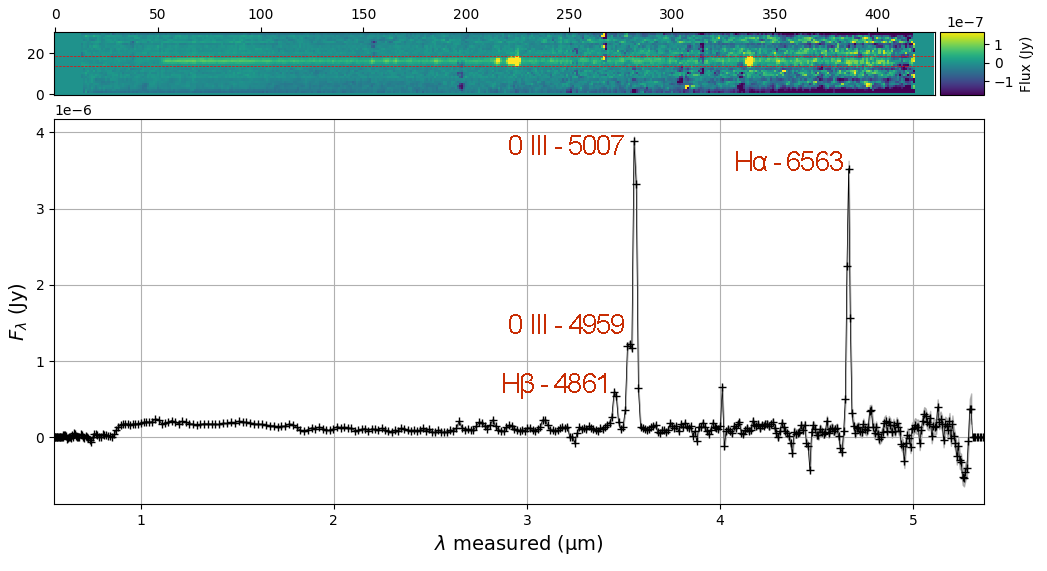
\includegraphics[width=\textwidth]{assets/P5_s01518_extracted.png}
\end{figure}

\begin{figure}
  \centering
     \begin{subfigure}[b]{0.3\textwidth}
         \centering
         
\includegraphics[width=\textwidth]{assets/paris-saclay.png}
     \end{subfigure}
     \hfill
     \begin{subfigure}[b]{0.3\textwidth}
         \centering
         
\includegraphics[width=\textwidth]{assets/lam.png}
     \end{subfigure}
\end{figure}

\newpage
\begin{center}
  \vspace*{\fill}

  Déclaration d'intégrité relative au plagiat \\

  

  Je soussigné \textbf{Dewachter Tim} certifie sur l'honneur : \\

  \begin{itemize}
    \centering
    \item Que les résultats décrits dans ce rapport sont l'aboutissement de mon travail ;\\
    \item Que je suis l'auteur de ce rapport ;\\
    \item Que je n'ai pas utilisé des sources ou résultats tiers sans clairement les citer et les référencer selon les règles bibliographiques préconisées.\\
  \end{itemize}

  Je déclare que ce travail ne peut être suspecté de plagiat. \\


  Date : \today\\

  

  Signature : Dewachter

  \vspace*{\fill}
\end{center}
\newpage

\tableofcontents

\newpage

\section{Abstract}

\textit{By establishing a new method of background subtraction on NIRSpec MOS data, we aim to prevent the negative traces that can be visible on some spectra treated by the basic pixel-per-pixel subtraction used by the JWST pipeline. This will allow us to detect secondary sources hidden in the background. The algorithm is based on an approximation of the background spectrum using a spline. This new post-calibrations data will then be analyzed using CIGALE in order to extract physical parameters such as redshift, metallicity or star formation rate.}

\section{Introduction}

\subsection{Contexte}

\begin{wrapfigure}{r}{10cm}
  \centering
  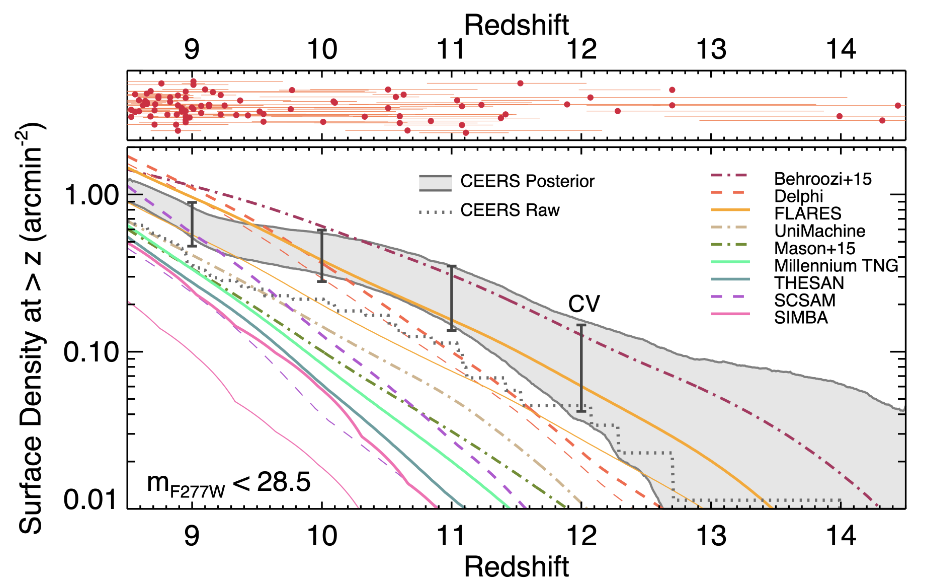
\includegraphics[scale=0.5]{assets/ceers_number_galaxies.png}
  \caption{Comparaisons modèles - données de la densité du nombre de galaxies en fonction du redshift. En haut, les différents \textit{redshifts} mesurés avec leurs incertitudes. En bas, Les traits colorés représentent différents modèles pré-JWST, tandis que la zone grisée représente les données obtenues par le programme CEERS. Seuls 2 modèles semblent en accord avec les données. \customcite{2023arXiv231104279F}}
  \label{fig:densite_galaxies}
\end{wrapfigure}

En seulement 2 ans d'opérations, le \gls{jwst} nous a déjà ouvert de nombreuses portes jusqu'alors inaccessibles, et cela dans de multiples branches de l'astrophysique. Grâce à ses instruments spectroscopiques et sa sensibilité à l'infrarouge proche et moyen, il est désormais possible de sonder l'univers comme jamais auparavant. Parmi les objectifs que l'on souhaite accomplir avec ce télescope, l'un d'eux est l'étude de la formation des galaxies à l'époque de la réionisation, de l'apparition des métaux au sein de celles-ci, et de la recherche des hypothétiques Populations III, constituées d'étoiles de métallicité nulle, formées par le gaz primordial d'Hydrogène et d'Hélium purs.

Ce nouvel horizon sur l'univers lointain nous permet de remonter l'histoire de l'univers comme jamais auparavant. En effet, la lumière ayant une vitesse finie, les photons nous arrivant maintenant depuis ces galaxies ont en réalité été émis longtemps dans le passé. Regarder loin dans l'espace est donc équivalent à remonter dans le temps. À cela s'ajoute également l'expansion de l'univers, qui a pour conséquence le décalage vers le rouge du spectre lumineux de ces objets lointains (on parle de \textit{redshift} $z$).

D'ores et déjà, de nombreux résultats remettent en question nos modèles précédemment établis. Notamment, il semblerait qu'il existe bien plus de galaxies dans l'univers jeune que ce que l'on pensait jusqu'à présent \parencite{2023arXiv231104279F} (voir figure \figref{fig:densite_galaxies}). Un autre résultat remarquable est la découverte d'un potentiel candidat de Population III \parencite{2023arXiv230600953M}, où une raie d'He II à $\lambda = 1640 \text{\r{A}}$ semble indiquer qu'un nuage de gaz à $z = 10.6$ s'est retrouvé ionisé par des étoiles de Pop III. 

Ainsi, dans les années à suivre, il est certain que de nouvelles contraintes vont pouvoir être posées sur les modèles de formation des premières galaxies et sur l'évolution de leur metallicité grâce au JWST.

\subsection{La poussière et les métaux}

\begin{figure}
  \centering
     \begin{subfigure}[t]{0.45\textwidth}
         \centering
         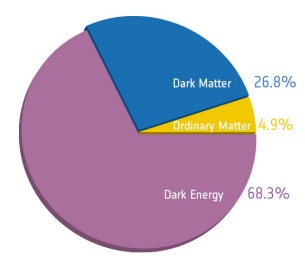
\includegraphics[width=1.2\textwidth]{assets/planck_cosmic_chart.jpg}
         \caption{Composition de la masse de l'univers. La matière baryonique représente $\sim 4.2\%$. \customcite{cosmological_composition}}
         \label{fig:cosmological_composition}
     \end{subfigure}
     \hfill
     \begin{subfigure}[t]{0.45\textwidth}
         \centering
         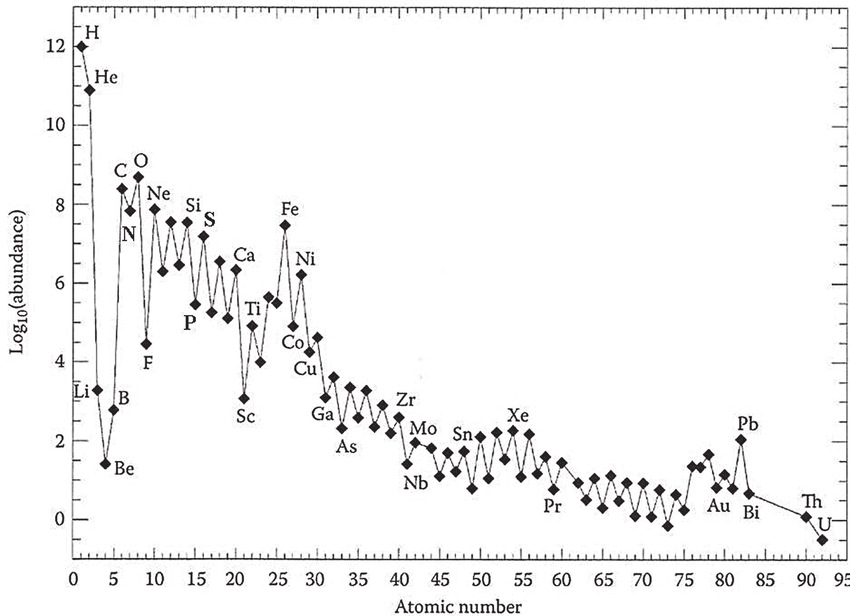
\includegraphics[width=\textwidth]{assets/Plot-showing-the-average-cosmic-abundance-of-elements-as-a-function-of-their-atomic.png}
         \caption{Abondance cosmique des différents éléments dans l'univers. L'axe des ordonnées est l'abondance telle qu'elle est définie dans l'équation \ref{eq:abundance}. \customcite{cosmic_abundance}}
         \label{fig:heavy_elements}
     \end{subfigure}
\end{figure}

En astrophysique, tout élément chimique plus lourd que l'hydrogène et l'hélium est dit métallique. En effet, lors des 20 premières minutes après le big bang, durant la nucléosynthèse primordiale, les isotopes d'hydrogène, d'hélium et une faible quantité de lithium furent les seuls noyaux formés \parencite{2017IJMPE..2641002C}. Tout élément plus lourd est apparu bien après, soit lors de la nucléosynthèse stellaire, soit lors d'événements cosmiques majeurs, tels que des supernovae ou des fusions de trous noirs ou d'étoiles à neutrons. Bien qu'à l'échelle humaine, ces éléments peuvent paraître abondants (carbone, oxygène et azote, ensembles avec l'hydrogène, sont les briques de base de la vie telle qu'on la connait), ils ne représentent qu'une infime partie de la masse de l'univers (la matière baryonique représente $4.2 \%$ de la masse totale \parencite{2024JCAP...06..006S}, les métaux représentent $\sim 2\%$ de la masse baryonique, soit $\sim 0.08\%$ de la masse totale.) (voir \figref{fig:cosmological_composition} et \figref{fig:heavy_elements}).

On mesure la métallicité en utilisant divers indicateurs. Le premier est la fraction de masse des éléments lourds rapportée à la masse totale,

\begin{equation}
  Z = \sum_{A > He} \frac{m_A}{M_{total}}
\end{equation}

qui peut se déterminer à partir de la fraction de masse d'Hydrogène $X = \frac{m_H}{M_{total}}$ et d'Hélium $Y = \frac{m_{He}}{M_{total}}$, en utilisant la relation $X + Y + Z = 1$. On mesure par exemple la métallicité du Soleil à $Z_\odot = 0.0134$ \parencite{2009ARA&A..47..481A}.

Cependant, lorsque la composition chimique exacte ne nous est pas accessible, on utilise souvent l'abondance relative en fer comme approximation de la métallicité, définie comme 

\begin{equation}
  [Fe/H] = \log(\frac{N_{Fe}}{N_H}) - \log(\frac{N_{Fe, \odot}}{N_{H, \odot}})
\end{equation}

où $N_{X}$ correspond au nombre d'atomes $X$ et $\odot$ traduit la mesure de cette valeur dans le cas du Soleil.

Un autre moyen d'estimer la métallicité est une mesure absolue du rapport entre la quantité d'oxygène sur la quantité d'hydrogène, appelée abondance.

\begin{equation}
  \label{eq:abundance}
  12 + \log{\frac{N_O}{N_H}}
\end{equation}

Ces rapports de quantités d'atomes peuvent être établis à partir de l'intensité des raies d'émission dans le spectre d'une galaxie, à condition de disposer au préalable d'un modèle des émissions stellaires qui viennent exciter les différents éléments.\\

À partir de ces atomes métalliques se forment alors les poussières, des grains de l'ordre du micron. Absorbant la lumière visible et ultraviolette avant de réémettre l'énergie ainsi accumulée dans l'infrarouge, maintenant la poussière à des température de l'ordre de $10 - 100K$ \parencite{Astrophysics-of-the-Diffuse-Universe}, faute de quoi la condensation et nucléation des grains dans le gaz en poussières plus grosses ne pourraient pas avoir lieu.

Une catégorie notable dans la famille des poussières sont les hydrocarbures aromatiques polycycliques, ou \gls{pah}, formés de cycles hexagonaux de carbone et d'hydrogène. Leur formation n'est donc uniquement possible que dans des nuages riches en carbone. Les grains de poussières sont également formés de silicates (silicium et oxygène) et de diverses glaces (d'eau, carbonique). La présence de poussière est alors intrinsèquement liée à la présence de métaux dans le nuage de gaz.

En plus de l'absorption dans l'UV-Visible et émission dans l'IR décrite plus haut, les grains peuvent également polariser la lumière les traversant, et l'asymétrie de leur structure leur donne accès à des transitions ro-vibrationnelles, également dans l'infrarouge.\\

\begin{figure}[!h]
  \centering
  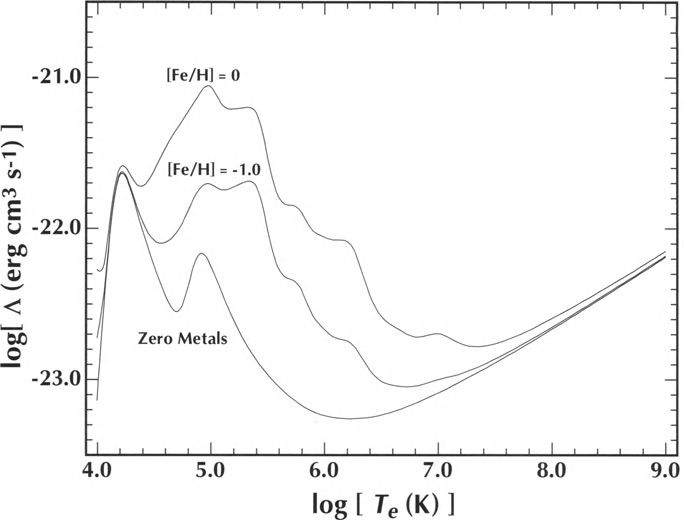
\includegraphics[scale=1.2]{assets/cooling.jpg}
  \caption{Fonctions de refroidissements en fonction de la métallicité. On remarque, dans le cas d'une métallicité nulle, 2 pics correspondants à l'hydrogène et l'hélium, tandis que dans le cas d'une métallicité non nulle, d'autres pics apparaissent pour des températures plus élevées, correspondants chacuns à des éléments plus lourds. Le refroidissement est alors plus efficace. Le comportement commun pour $\log(T_e) > 7$ est dû au rayonnement de freinage \textit{Bremsstrahlung} \customcite{Astrophysics-of-the-Diffuse-Universe}.}
  \label{fig:cooling}
\end{figure}

La présence de métaux et de poussière dans un nuage de gaz a donc une conséquence fondamentale sur celui-ci : un refroidissement plus efficace. En effet, les nouvelles transitions électroniques offertes par ces éléments lourds, combinées aux excitations créées par les collisions, permettent à la fonction de refroidissement $\Lambda(T_e,Z_A) = \frac{\dot{Q}}{n_e n}$ ($T_e$ la température électronique du plasma, $Z_A$ la charge de l'atome $A$ du plasma, $n_e$ et $n$ la densité électronique et densité de l'atome $A$, $\dot Q$ le taux de refroidissement du gaz), de voir apparaître de nouveaux pics (\figref{fig:cooling}), permettant donc un meilleur refroidissement à des températures plus élevées.\\

Ce manque de refroidissement a une conséquence notable : la formation d'étoiles massives. En effet, le nuage de gaz initial ayant plus de difficultés à se refroidir, celui-ci se fragmente moins (mais se fragmente tout de même, contrairement à ce qui était pensé il y a encore quelques années, voir \cite{Tan_2004}) et les fragments forment donc des étoiles plus massives, qui par conséquent vivent peu de temps \parencite{2023ARA&A..61...65K}. Ces premières étoiles de métallicité nulle, dites de Population III n'ont à ce jour jamais été observées. Leur découverte aurait un impact majeur sur l'étude de la formation des galaxies, notamment dans la compréhension de l'apparition des métaux dans celles-ci.

\subsection{Problématiques et Objectifs}

Comment peut-on utiliser la spectroscopie comme outil pour sonder les paramètres physiques des premières galaxies ?\\

Nous allons par la suite traiter ce problème en 2 parties.

Tout d'abord, nous étudierons le code de traitement des données du \gls{jwst} dans le but de modifier son algorithme de soustraction du fond, afin d'en extraire les éventuels faibles spectres de sources secondaires jusqu'alors dissimulés dans le fond.

Ensuite, nous étudierons ces différents spectres via \gls{cigale} afin d'en déterminer les paramètres physiques, tels que leur redshift, leur metallicité ou leur taux de formation stellaire.

\section{Méthodologie}

\subsection{JWST et NIRSpec}

\begin{figure}
  \centering
     \begin{subfigure}[b]{0.45\textwidth}
         \centering
         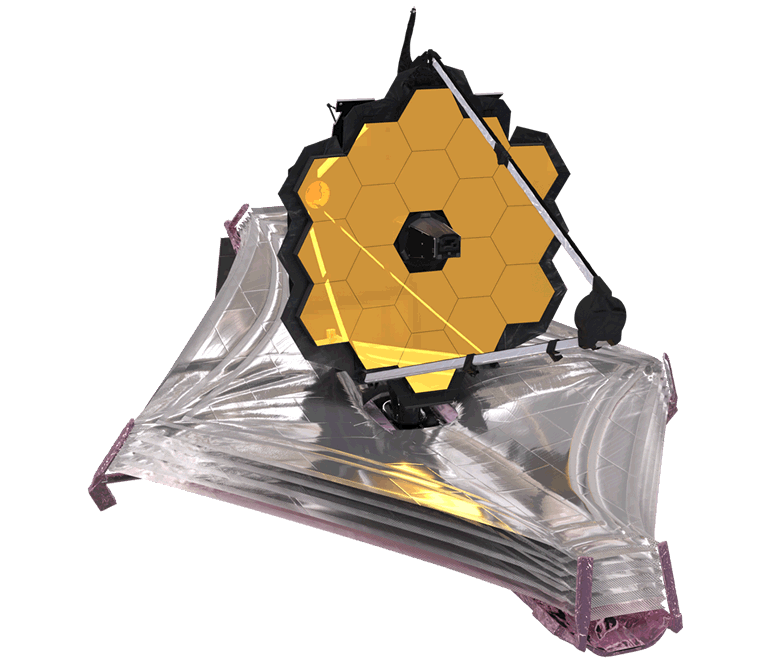
\includegraphics[width=\textwidth]{assets/JWST_spacecraft_model_3.png}
         \caption{Rendu 3D du \gls{jwst}. \customcite{jwst_nasa}}
         \label{fig:jwst}
     \end{subfigure}
     \hfill
     \begin{subfigure}[b]{0.45\textwidth}
         \centering
         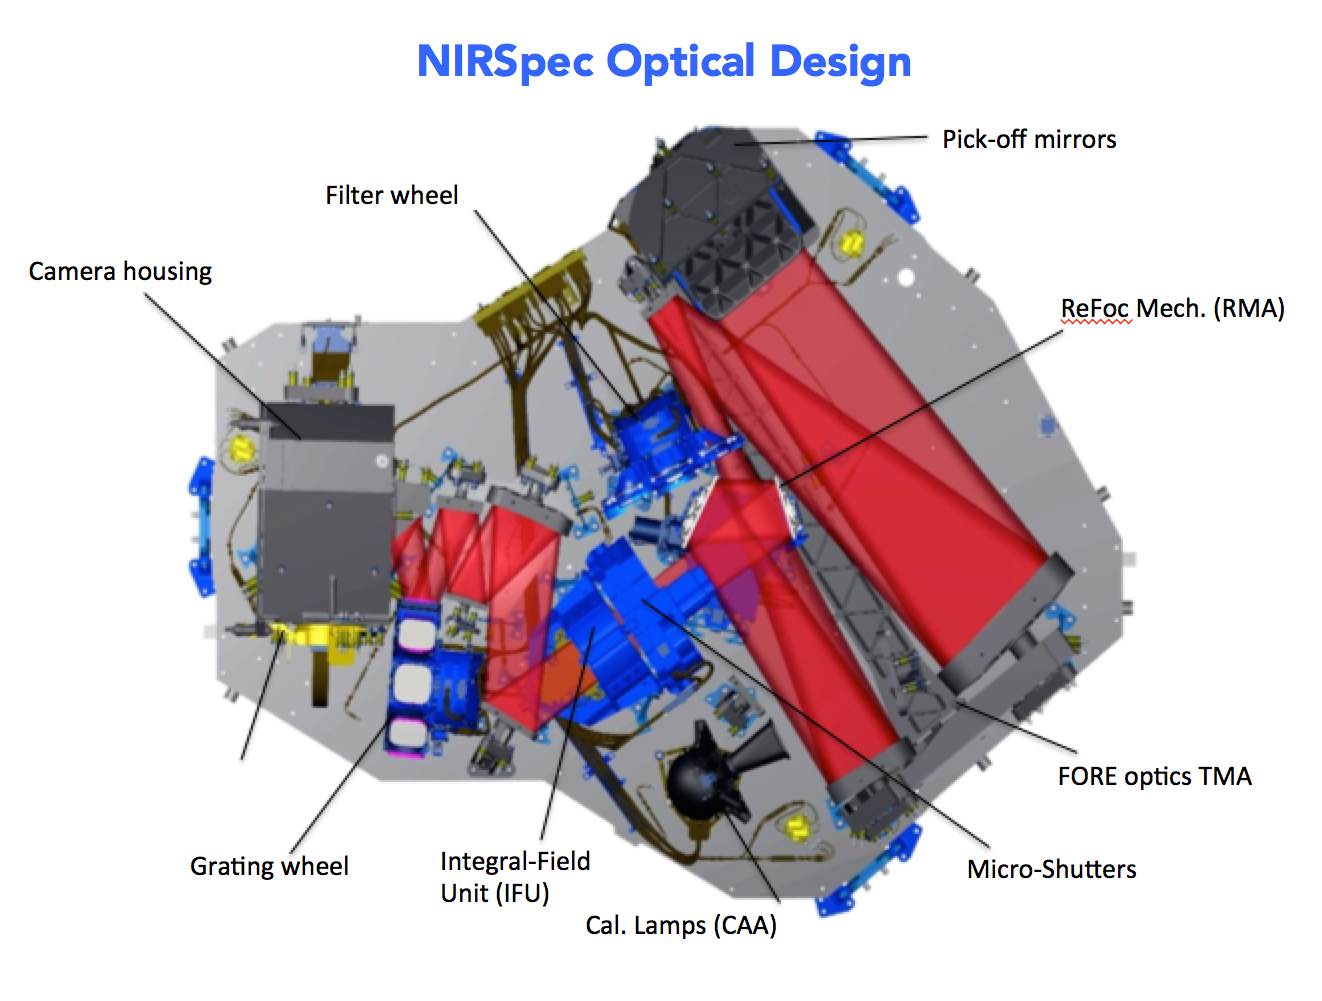
\includegraphics[width=\textwidth]{assets/NIRSpec_Optical_design.png}
         \caption{Schéma des optiques de \gls{nirspec}. \customcite{nirspec}}
         \label{fig:nirspec}
     \end{subfigure}
\end{figure}

Le \gls{jwst} est un télescope spatial de 6.5 mètres de diamètre équivalent, en orbite autour du point de Lagrange L2, et actif depuis juillet 2022 \parenciteauthortitle{jwst_website}. Sa sensibilité dans l'infrarouge en fait un outil remarquable pour observer l'univers jeune. En effet, de par l'expansion de l'univers, la lumière des objets lointains se retrouve décalée vers le rouge : il s'agit du \textit{redshift} $z$, défini comme 

\begin{equation}
    1 + z = \frac{\lambda_{obs}}{\lambda_{rest}}
\end{equation}

Avec $\lambda_{obs}$ la longueur d'onde observée, et $\lambda_{rest}$ la longueur d'onde dans le référentiel de la source (au repos). Ainsi, regarder loin dans l'espace est équivalent à regarder loin dans le passé et nécessite d'observer à des longueurs d'ondes de plus en plus grandes. Puisque l'on s'attend à ce que les premières étoiles soient massives, elles devraient donc briller dans le bleu-ultraviolet. Aux \textit{redshifts} étudiés, ces longueurs d'ondes se retrouvent alors décalées dans l'infrarouge proche.

\begin{figure}[!h]
  \centering
  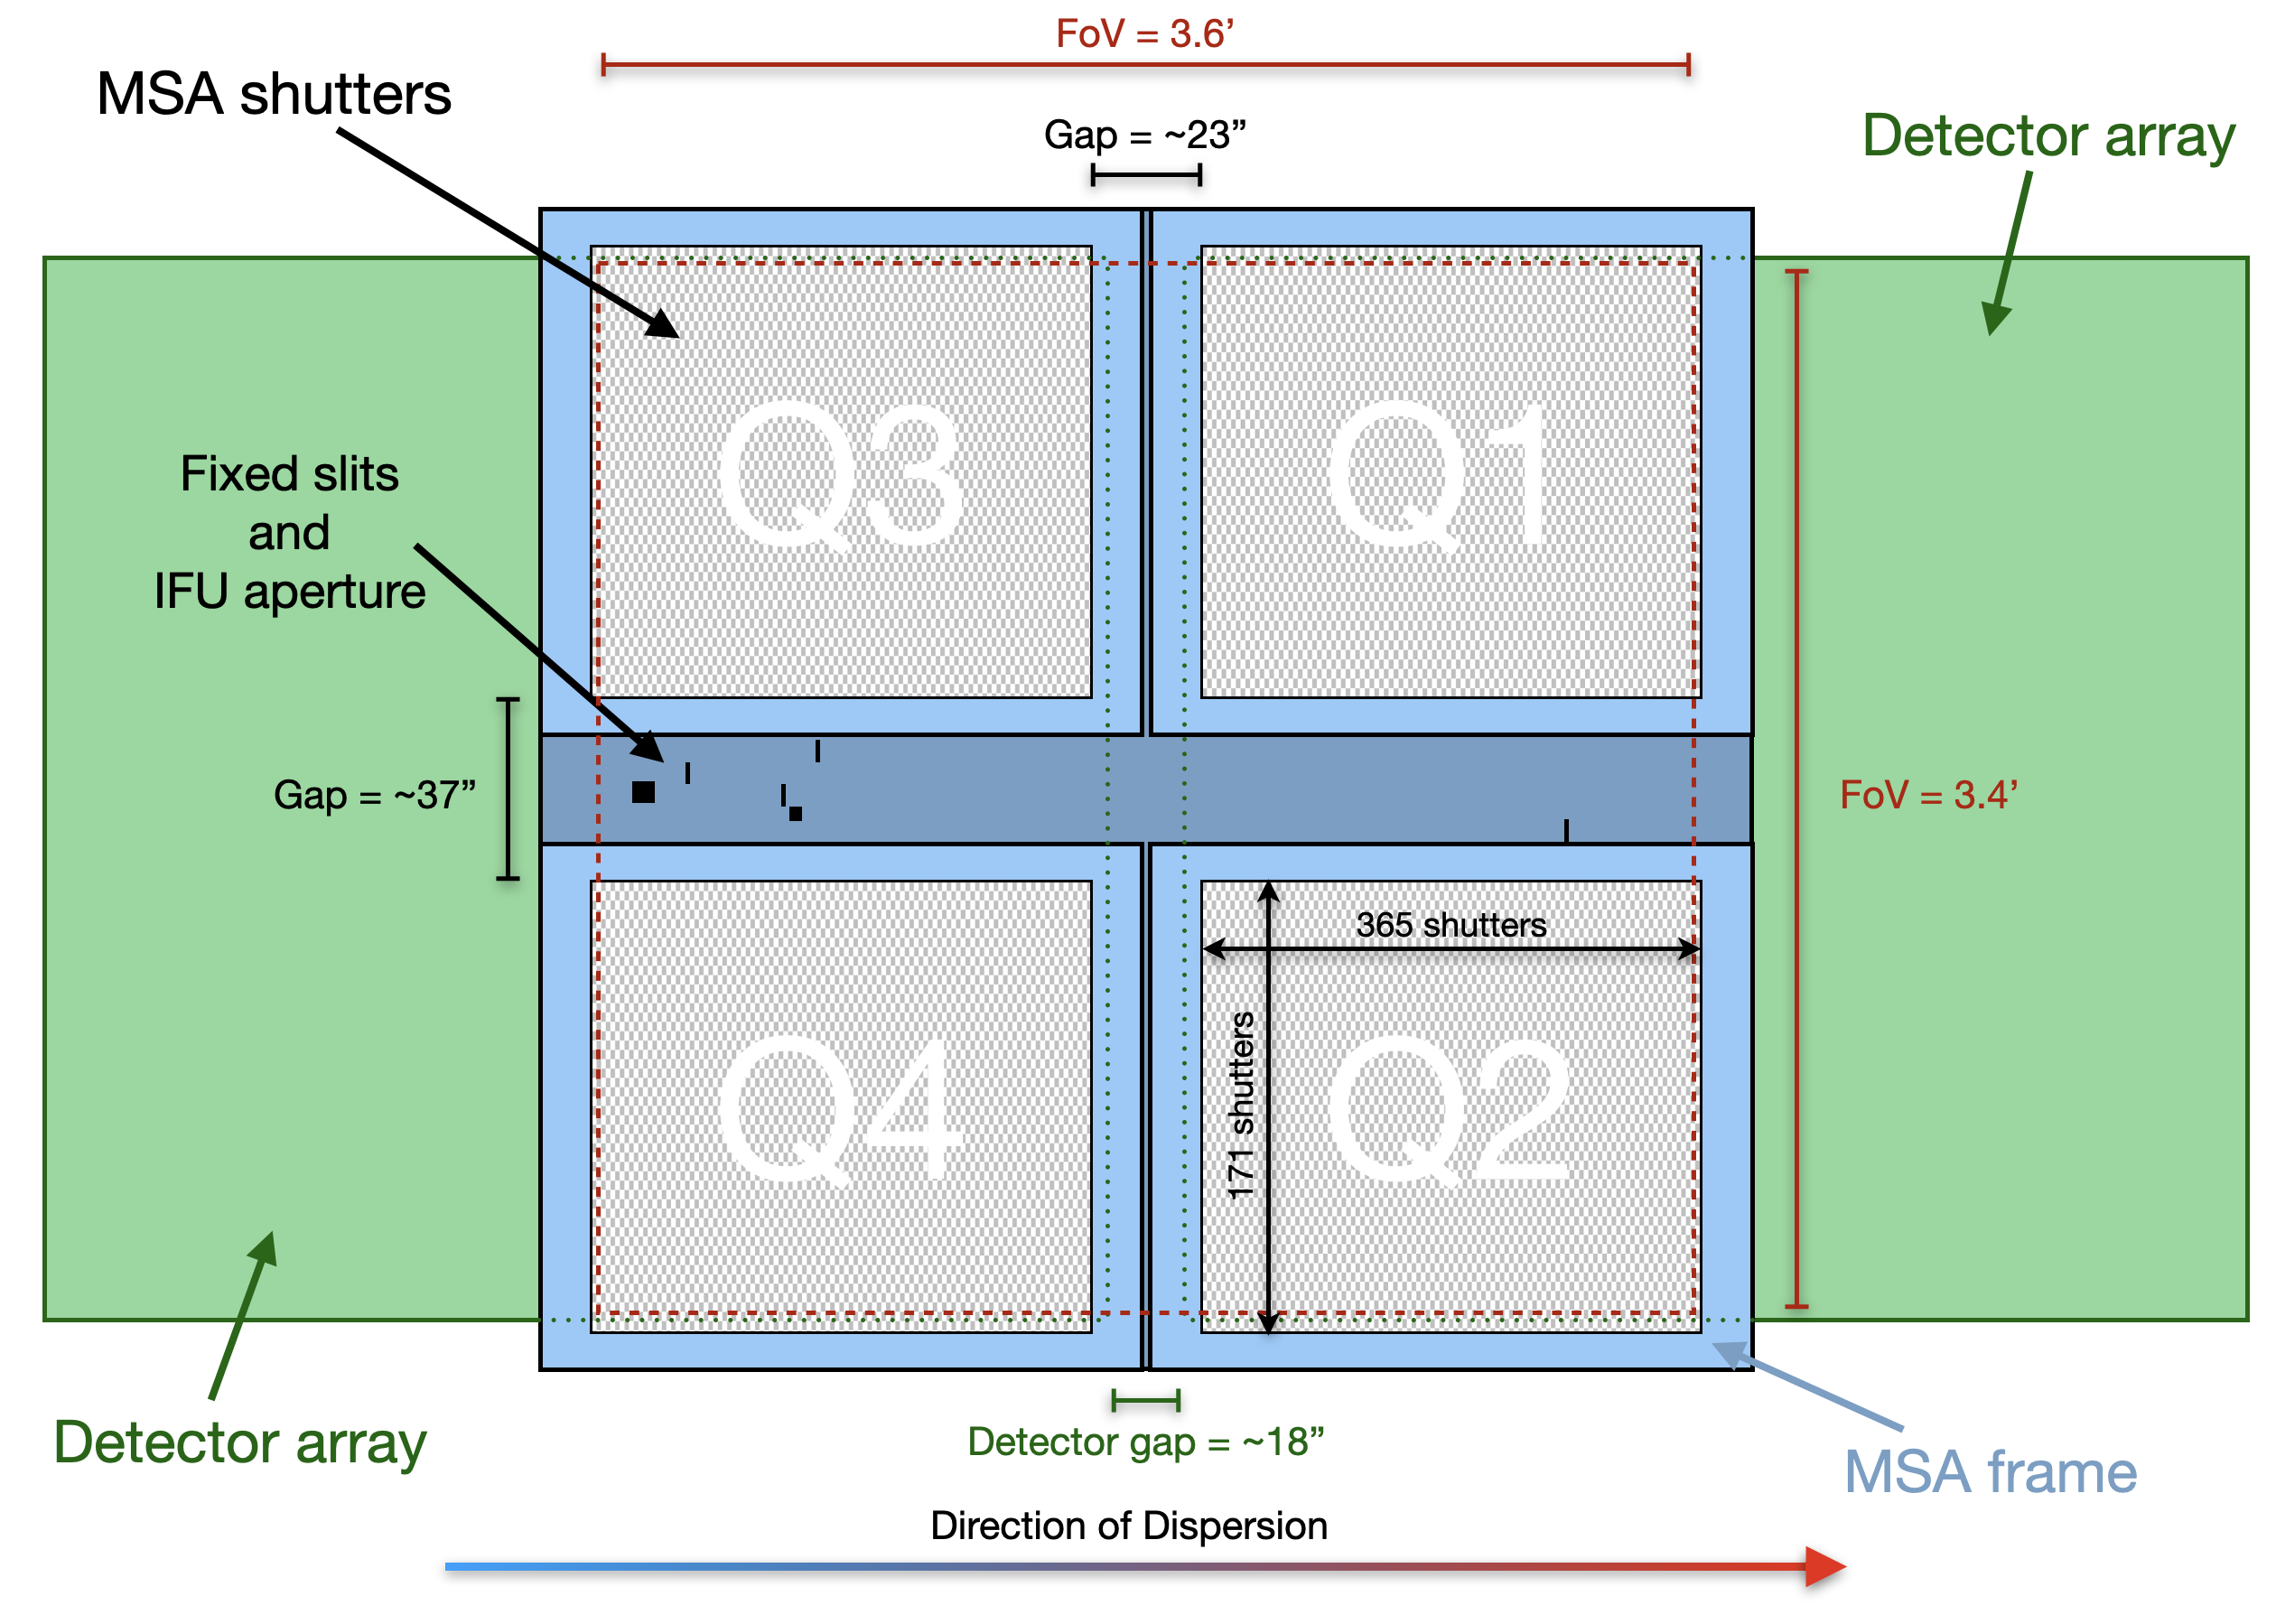
\includegraphics[scale=0.4]{assets/msa_ds_new.png}
  \caption{Disposition de MSA dans le plan focal de NIRSpec. \customcite{2022A&A...661A..81F}}
  \label{fig:msa_shutter}
\end{figure}

Parmi les instruments du \gls{jwst}, \gls{nirspec} est un spectromètre sur la bande 0.6 - 5.3  µm, disposant de 3 modes de résolution : PRISM ($R \sim 100$), medium grating ($R \sim 1000$), high grating ($R \sim 2700$) \parenciteauthortitle{nirspec}. L'un des atouts principaux de \gls{nirspec} est son \gls{msa}, une grille de près de 250 000 obturateurs, couvrant une surface de 3.6' x 3.4' sur le ciel, chacun pouvant être individuellement ouvert ou fermé \parenciteauthortitle{msa} (voir \figref{fig:msa_shutter}). Ceci permet d'observer dans le mode \gls{mos}. Comme son nom l'indique, la spectroscopie multi-objets permet d'extraire le spectre de plusieurs objets dans un même champ, mais la grille d'obturateurs apporte également un outil fondamental dans l'extraction des spectres : la soustraction du fond.\\

Nous travaillerons ici sur des données \gls{nirspec} du Programme de \gls{ceers}, disponibles sur la base de données MAST \parenciteauthortitle{portal_mast} (\textit{Proposal ID : 1345}), notamment les observations P4, P5, P7, P8, P11, P12, avec comme résolution PRISM.

\subsection{Fond, \textit{Nodding} et \textit{Slitlet}}

Lorsqu'on s'intéresse à des sources de faible brillance, la densité de flux mesurée peut rapidement se trouver dominée par les émissions du fond. Que ce soit le fond diffus infrarouge, produit par des sources extragalactiques non résolues, la lumière zodiacale, produite par la poussière interplanétaire, le rayonnement de la Voie Lactée ou l'émission thermique du JWST lui-même, l'infrarouge est un domaine facilement parasité par des signaux indésirables \parenciteauthortitle{jwst_background}. De plus, la nature de ses composantes fait de ce fond un signal anisotrope. Il n'est donc pas si simple d'en établir un modèle universel à soustraire de façon systématique. Les composantes du fond sont présentées \figref{fig:background_jwst} en fonction de la longueur d'onde : 

\begin{figure}[!h]
  \centering
  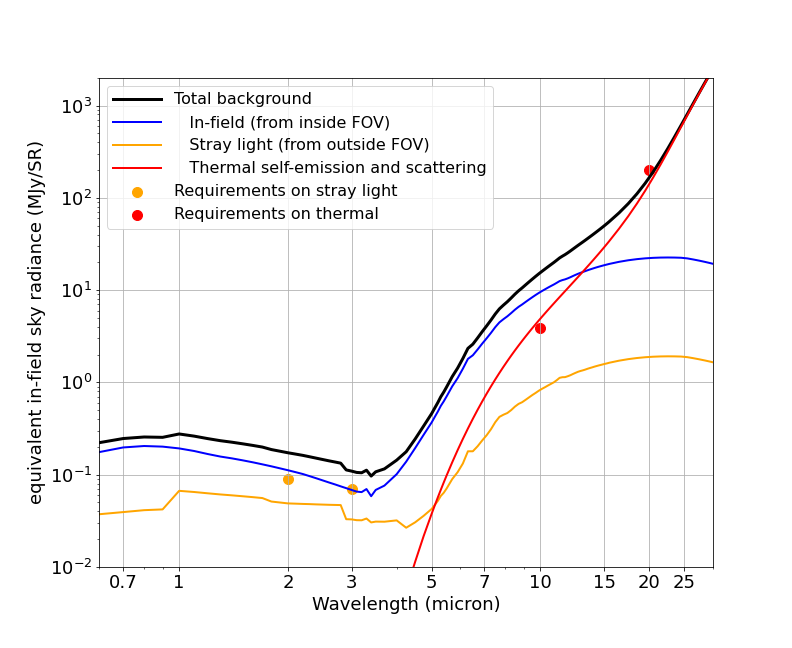
\includegraphics[scale=0.55]{assets/background_jwst.png}
  \caption{Densité de flux par unité d'angle solide reçu par le JWST en fonction de la longueur d'onde. On remarque qu'à mesure que $\lambda$ augmente, l'émission thermique du télescope domine. \customcite{jwst_background}}
  \label{fig:background_jwst}
\end{figure}


Cependant, il reste tout de même envisageable de corriger ce signal parasite. En effet, en ouvrant les obturateurs à proximité de celui imageant la source, il devient possible d'extraire le fond localement autour de celle-ci, que l'on peut alors lui soustraire.

La configuration habituelle consiste en l'ouverture de 3 obturateurs dans la direction perpendiculaire à la direction de dispersion. Dans un souci de cohérence avec la documentation du pipeline, on décrira par la suite cet ensemble de 3 obturateurs comme un \textit{slitlet}. On réalise alors 3 expositions, chacune en orientant le télescope de façon à avoir la source dans un obturateur différent : il s'agit du \textit{nodding}. Ce mouvement entre chaque exposition offre également un autre avantage au travers du \textit{dithering}. La \gls{psf} de \gls{nirspec} est effectivement de $0.08 ''$ à $\lambda = 2.46 \mu m$ \parencite{10_1051_0004_6361_202142663}. 
Comme $PSF \propto \lambda$, on a une \gls{psf} variant de $0.02 ''$ à $0.17''$ le long de la plage de longueurs d'ondes observables. Comme la taille d'un pixel est $\sim 0.1''$ dans la direction spatiale, la \gls{psf} est sous échantillonnée presque partout. Le \textit{dithering} permet alors d'améliorer cet échantillonnage par des corrections sub-pixels, mais également de s'affranchir des éventuels pixels défectueux ou des rayons cosmiques.

On résume ceci dans la \figref{fig:msa_slitlet}.


\begin{figure}[H]
  \centering
  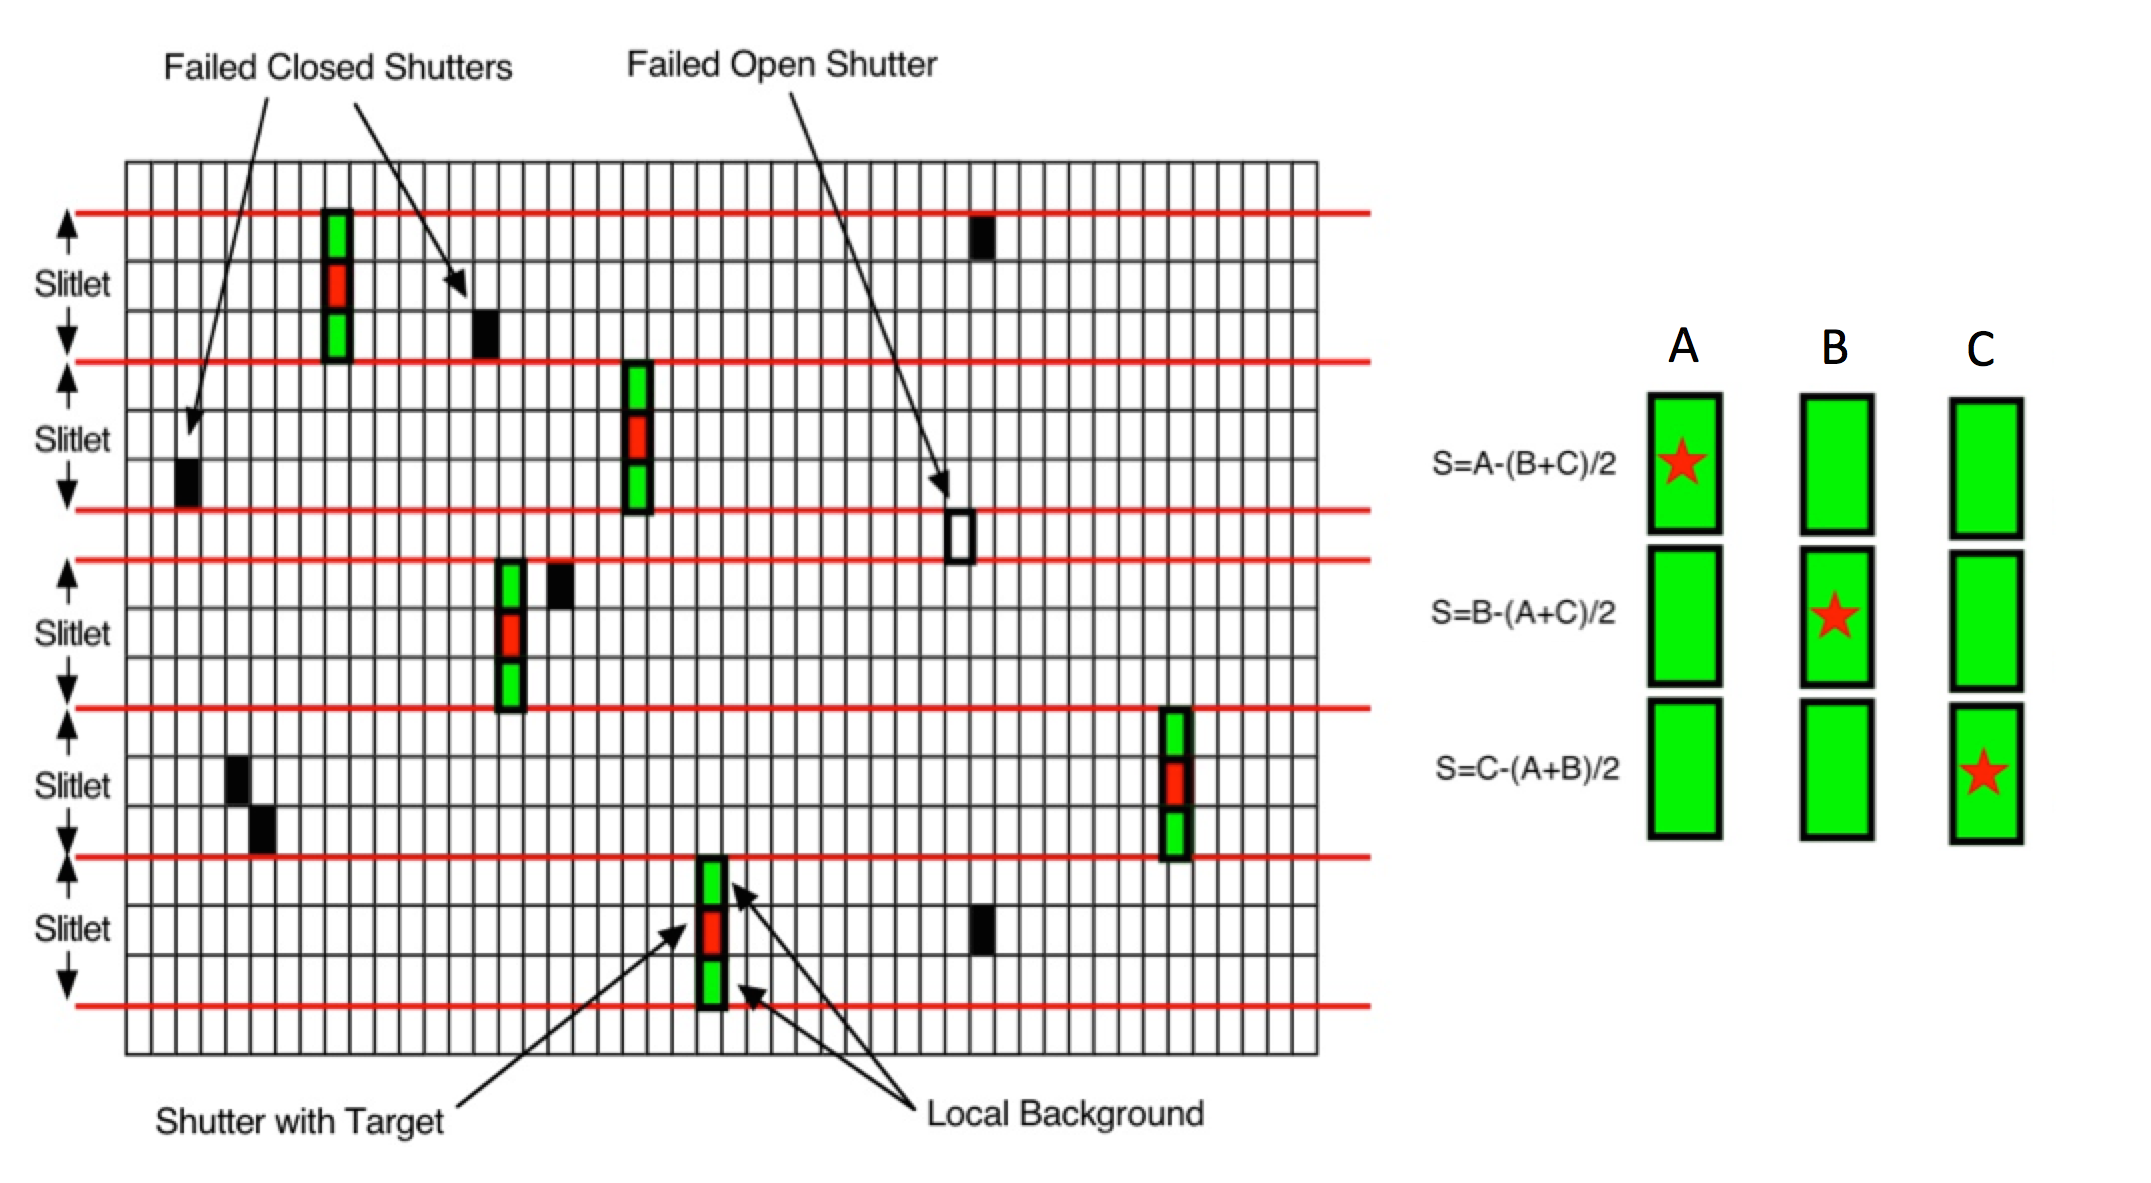
\includegraphics[scale=0.2]{assets/MSA_sky_strategy.png}
  \caption{Schéma de MSA et de \textit{slitlets}. On réalise des séries de 3 images, chacune ayant la source dans un obturateur différent, et on utilise les 2 obturateurs restants pour déterminer le spectre du fond. \customcite{mos}}
  \label{fig:msa_slitlet}
\end{figure}

\subsection{Le pipeline JWST}

Le code permettant de traiter les données reçues du JWST, appelé pipeline (\figref{fig:jwst_pipeline}), se décompose en 3 grandes étapes, celles-ci étant de plus en plus spécifiques aux types de données que l'on cherche à étudier à mesure que l'on progresse dans le pipeline.

Ainsi, dans notre cas, les 3 étapes sont telles que :\\


\begin{minipage}{.45\linewidth}
  \begin{itemize}[left=0cm]
    \item \textbf{Detector 1} : Applique les corrections au niveau du détecteur, tel que le masquage des pixels morts/chauds et des rayons cosmiques, la linéarisation du nombre de détections par seconde, la suppression du biais et du courant d'obscurité... Cette étape est la même pour tous les instruments du \gls{jwst}. (cf. \figref{fig:rate_file} le fichier en sortie de cette étape)
    \item \textbf{Spectroscopy 2} : Applique des modifications optiques, telles que la correction de champ plat et des pertes de lumières liées aux barres séparant les obturateurs, mais calibre également la photométrie et les données \gls{wcs}, associant à chaque pixel des coordonnées spatiales et spectrales. C'est ici que les images de chaque \textit{slitlets} sont extraites de l'image initiale et que la soustraction du fond s'applique.
    \item \textbf{Spectroscopy 3} : Combine plusieurs expositions entre elles, appliquant ainsi le \textit{dithering} / \textit{nodding} discuté plus tôt, ré-échantillonne les images 2D et extrait les spectres 1D de celles-ci.
  \end{itemize}
  \end{minipage}
  \hfill
  \begin{minipage}{.5\linewidth}
  \centering
  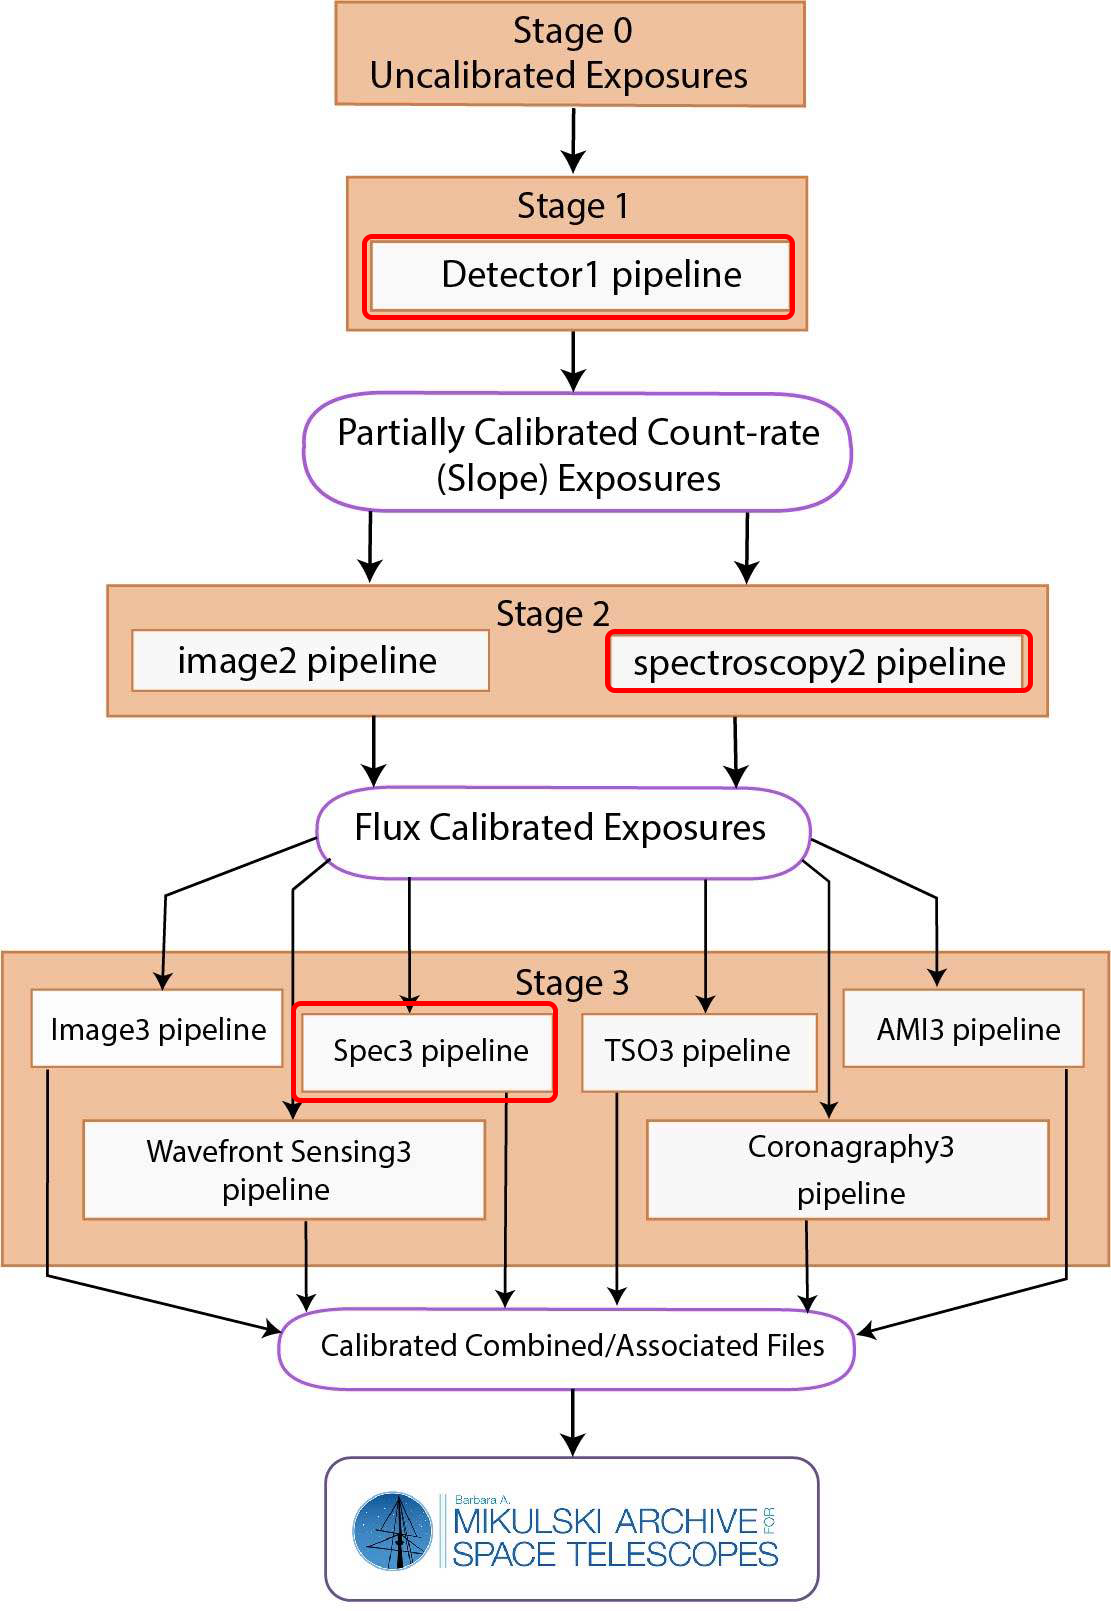
\includegraphics[scale=0.15]{assets/jwst_pipeline.jpg}
  \captionof{figure}{Schéma des différentes étapes du pipeline. Les étapes adaptées à nos données sont encadrées en rouge.\customcite{jwst_pipeline}}
  \label{fig:jwst_pipeline}
  \end{minipage}


  \begin{figure}[H]
    \centering
    \begin{overpic}[width=1\textwidth]{assets/rate_file_illustrated.png}
      % The coordinates (x, y) specify the position of the caption text.
      % For example, (20,80) would place the caption at 20% from the left and 80% from the bottom.
      \put(52.5,13){%
          \parbox{8cm}{
            \fontsize{11}{12}\selectfont Image de \gls{nirspec} en sortie de l'étape 1 du pipeline. On peut y observer des taches lumineuses correspondant aux ordres 0 de diffraction (vert), des larges bandes au milieu formées par des obturateurs toujours ouverts, utilisés lors du mode Fixed Slit (bleu), ainsi que des bandes plus fines, parfois regroupées par 3, parfois isolées lorsqu'un obturateur reste accidentellement ouvert.
          }
      }
    \end{overpic}
    \caption{}
    \label{fig:rate_file}
  \end{figure}

  \subsubsection{Soustraction du fond par défaut}

  Par la suite, on appelle \textit{bande} l'image d'un obturateur à travers le système optique, c'est à dire la tâche lumineuse sur l'image pour laquelle une direction correspond à la dispersion spectrale, et l'autre à l'étalement spatial.\\

  Dans le cas de données \gls{nirspec} \gls{mos}, la soustraction du fond se fait pixel par pixel, lors de l'étape 2 du pipeline. Sur chaque \textit{slitlet}, pour une exposition donnée, on considère les 2 expositions restantes comme du signal de fond, on les moyenne donc avant de les soustraire à l'image initiale. Cette étape est décrite sur la \figref{fig:msa_slitlet}

  Cette méthode a l'avantage majeur de permettre de soustraire le fond localement autour de la source. Cependant, elle se heurte à un problème dans le cas où la source est suffisamment étendue pour être visible depuis un des obturateurs de fond, ou dans celui où la source est mal centrée dans l'obturateur principal. Ceci devient en revanche plus intéressant dans le cas où une autre source suffisamment brillante se situe dans le champ d'un des obturateurs de fond. Dans chacun de ces scénarios, le spectre de "fond" n'en est plus réellement un : on observe une sur-correction du spectre de l'objet. Les raies d'émission sont atténuées sur la bande de signal et des raies inversées apparaissent sur les autres bandes, en raison de la soustraction. C'est ce que l'on observe sur la \figref{fig:negative_trace} : les bandes au-dessus et en dessous de la bande principale présentent un spectre négatif. Cette sur-correction a également pour conséquence de cacher toute galaxie de faible luminosité se trouvant dans une des bandes du fond.\\
  
  \begin{figure}[H]
    \centering
    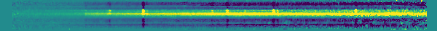
\includegraphics[scale=1.1]{assets/negative_trace_nirspec.png}
    \caption{Exemple d'une image 2D d'un spectre de \gls{nirspec} en fin de traitement classique. On observe clairement des spectres négatifs au-dessus et en dessous de la bande contenant le signal. Ceci est particulièrement visible à proximité des raies intenses.}
    \label{fig:negative_trace}
  \end{figure}

  Le pipeline offre également un autre algorithme, dit de master background, qui extrait puis combine les spectres de plusieurs obturateurs de fond, ailleurs dans le champ, avant de ré-interpoler le spectre en 2D et de le soustraire. Cette méthode, bien qu'offrant en général un meilleur rapport signal sur bruit, a le désavantage de perdre l'aspect local du fond qu'offre la soustraction pixel par pixel.

  \subsubsection{Soustraction du fond personnalisée}

  Nous allons ici chercher à établir une nouvelle méthode de soustraction du fond, combinant le meilleur signal sur bruit du master background avec la composante locale de la soustraction pixel par pixel. L'algorithme est comme suit :\\

  \begin{algorithm}[H]
    $raw$ = données à traiter \;
    Appliquer le stage 1 du pipeline sur $raw$ \;
    Appliquer le stage 2 du pipeline sur $raw$ jusqu'à l'étape Master Background \;
    Application temporaire des étapes FlatField, PathLoss, BarShadow, Photom, ResampleSpec \;
    \ForEach{\textit{Slitlet} dans $raw$}{
      \If{Nombre de shutters dans \textit{slitlet} = 3}{
        Moyenne spectrale de l'image dans la direction de dispersion \;
        Détermination des positions $y_i$ de chaque bande par ajustement de 3 profils gaussien \;
        \ForEach{$i \in [1,2,3] \; \& \; i \neq source$}{
          Extraction et moyenne spatiale des $z_j^i$, les 2 bandes de fond, centrée sur $y_i$, avec une étendue spatiale de 3 pixels \;
          Extraction et moyenne spatiale des $\lambda_j^i$, longueurs d'ondes associées \;
          Extraction et moyenne spatiale des $(\sigma_j^i)^2$, les variances sur $z_j^i$ associées \;          
         }
        Ajuster une spline $f(\lambda_j^i)$ aux données $z_j^i$, de degré $k=5$ et de facteur de lissage $s=0.01$ \;
        Créer une nouvelle image $Z_{(x,y)} = f(\lambda_{(x,y)})$ \;
        Appliquer les étapes inverses de ResampleSpec, Photom, BarShadow, PathLoss, FlatField \;
        Calcul des données traitées $trait\acute{e}e_{(x,y)} = raw_{(x,y)} - Z_{(x,y)}$ \;
        }
    }
    Appliquer les étapes suivantes du stage 2 du pipeline sur $trait\acute{e}e$\;
    Appliquer le stage 3 du pipeline sur $trait\acute{e}e$\;
  \end{algorithm}

\subsection{Analyse de l'algorithme}

La méthode décrite ici est basée sur celle utilisée lors de l'étape MasterBackgroundStep du pipeline \parenciteauthortitle{mos_master_background}.

\subsubsection{Calibration temporaire}

L'application temporaire des étapes \texttt{FlatField}, \texttt{PathLoss}, \texttt{BarShadow}, \texttt{Photom} et \texttt{ResampleSpec}, permet d'extraire les spectres de fond de façon plus efficace. Ces étapes sont inversées par la suite, une fois un modèle de fond calculé, cela dans le but de faciliter l'ajustement.

\begin{itemize}
  \item \textbf{FlatField} : Le \textit{Flat Field}, ou Champ Plat, permet de corriger les défauts optiques (débris sur les miroirs ou le détecteur, distorsions optiques...) ainsi que les variations de sensibilités de chaque pixel. Ces images de calibrations dépendent de la longueur d'onde, et il est donc nécessaire dans le cas de \gls{nirspec} d'en combiner et interpoler plusieurs afin de couvrir le domaine spectral observé. La correction est alors appliquée en divisant l'image de chaque \textit{slitlet} par le champ plat.
  \begin{equation}
    \mathsf{CORRECTION} = \mathsf{SCI} \; / \; \mathsf{FLAT} 
  \end{equation}

  \item \textbf{PathLoss} : Permet de compenser les pertes de lumière dans le système optique (taille finie des obturateurs, pertes de lumière en dehors du réseau).
  
  \item \textbf{BarShadow} : Compense les pertes liées aux barres séparant les obturateurs dans le cas de sources étendues.
  
  \item \textbf{Photom} : Traitement photométrique de l'image, où celle-ci passe de valeurs arbitraires en DN/s (comptage d'événements par seconde) à des valeurs physiques de densité de flux. Le facteur de conversion dépend de la longueur d'onde et est obtenu grâce à un tableau de référence, avant d'être interpolé aux longueurs d'ondes d'intérêt.\\
  
  À la fin de cette étape, une copie des données prétraitées est réalisée. C'est depuis cette copie que les étapes inverses seront appliquées par la suite.
  
  \item \textbf{ResampleSpec} : Ré-échantillone l'image de chaque \textit{slitlet} de façon à corriger toute déformation et rotation de l'image, tout en alignant la direction de dispersion spectrale sur l'axe horizontal et la direction spatiale avec l'axe vertical.
\end{itemize}

\begin{figure}[H]
  \centering
  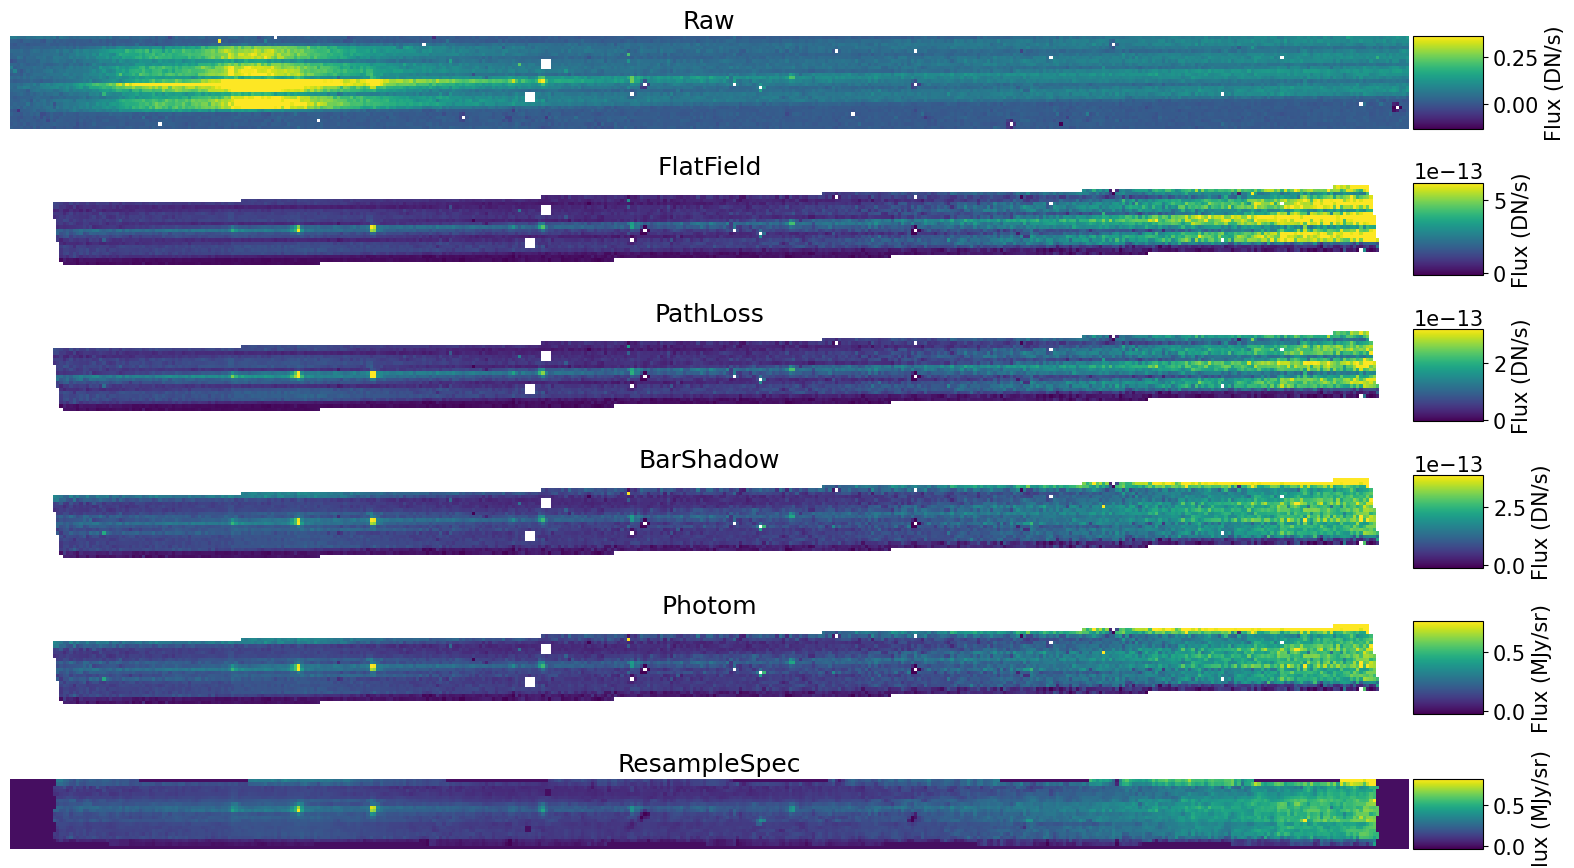
\includegraphics[scale=0.45]{assets/precal.png}
  \caption{La précalibration appliquée à l'image d'un \textit{slitlet}. On remarque que le traitement par \texttt{FlatField} corrige grandement le flux et est effectivement inégal selon la longueur d'onde, que \texttt{PathLoss} et \texttt{BarShadow} permettent de s'affranchir de l'ombre des barres sur l'image, que \texttt{Photom} permet le passage de $DN/s$ (le nombre de détections par seconde) vers des $MJy/sr$, et que \texttt{ResampleSpec} permet de redresser l'image. Les pixels blancs sont des pixels masqués par l'algorithme, car défectueux ou présence de rayons cosmiques.}
  \label{fig:precal}
\end{figure}


\subsubsection{Détermination des positions des bandes}

L'étape \texttt{ResampleSpec} nous permet d'être certains que la direction verticale sur l'image correspond à une dispersion spatiale, tandis que la direction horizontale correspond à l'étalement spectral. Pour discriminer la bande contenant le signal principal de celles contenant le spectre de fond, nous réalisons donc une moyenne spectrale, tronquée à $5\sigma$, afin de nous ramener à un problème à 1 dimension.\\

À ce profil, on ajuste alors une somme de 3 gaussiennes, censées modeliser l'apparence spatiale des 3 bandes (\figref{fig:profil_gauss}). Des 2 gaussiennes correspondant au fond, on récupère alors leurs positions, autour desquelles on réalise une extraction dans la direction spectrale sur l'image (\figref{fig:extraction}). On extrait alors également les longueurs d'ondes associées à chaque pixel ainsi que l'erreur sur la densité de flux. La fenêtre d'extraction utilisée est prise à 3 pixels de haut.

Pour chacune des bandes, on réalise alors une dernière moyenne, sur la direction spatiale, afin d'obtenir $z^i_j$ (tronqué à $5\sigma$), $\lambda^i_j$ et $\sigma^i_j$ (dans le cas de l'erreur, la moyenne se fait quadratiquement).

\subsubsection{Ajustement par une spline}

\begin{wrapfigure}{r}{.5\textwidth}
  \begin{minipage}{\linewidth}
    \centering\captionsetup[subfigure]{justification=centering}
    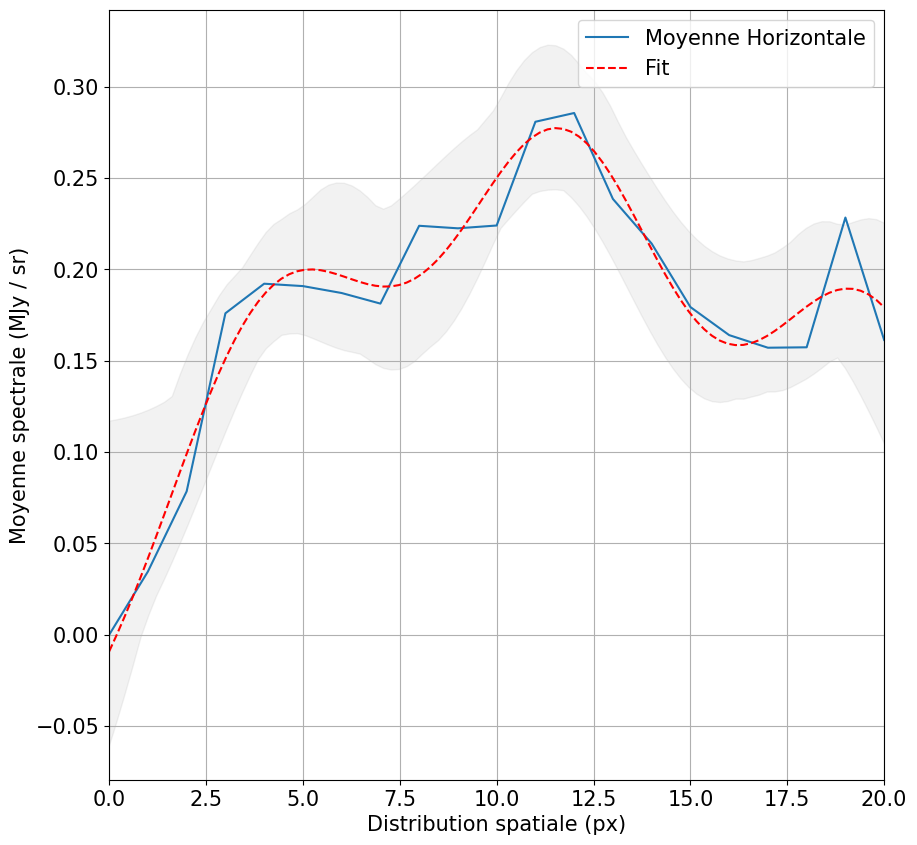
\includegraphics[width=0.9\linewidth]{assets/fit_gaussian.png}
    \subcaption{Profil de la distribution spatiale de l'image d'une \textit{slitlet} après avoir moyenné sur les longueurs d'ondes. On ajuste alors ce profil par 3 gaussiennes.}
    \label{fig:profil_gauss}
    \par
    \vfill
    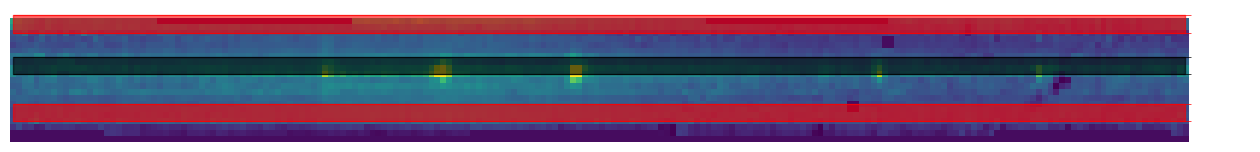
\includegraphics[width=\linewidth]{assets/extraction.png}
    \subcaption{Visualisation en rouge des zones d'extractions du fond et en noir de la zone du signal, qui ne nous intéresse pas ici.}
    \label{fig:extraction}
  \end{minipage}
\end{wrapfigure}

À présent que l'on dispose d'un ensemble de points $(\lambda, z)$, on cherche à trouver une fonction approximant $z = f(\lambda)$ de façon à ignorer les variations rapides et le bruit. Pour cela, on utilise la fonction \texttt{UnivariateSpline} du module \texttt{SciPy.interpolate}, afin d'ajuster un modèle de spline à nos données. Puisque les variations qui nous intéressent sont les basses fréquences, et que celles-ci peuvent parfois présenter plusieurs extrema, on choisira comme ordre de la spline le degré maximal, à savoir $k=5$ (cela signifie que les morceaux de polynômes servant à construire la courbe, seront au plus de degré 5). 

On dispose également d'un paramètre de lissage $s \geq 0$, qui quantifie le nombre de sous intervalles sur lesquels on définit les morceaux de polynômes. Plus $s$ est proche de 0, plus la fonction passera à proximité de chaque point, plus $s$ est grand, plus la fonction sera "lisse" et ne suivra que l'allure générale de la distribution des points. On choisit, assez arbitrairement, une valeur de $s=0.01$.

Il est possible que dans certains cas, l'ajustement de la spline échoue. L'algorithme baisse alors la valeur de $k$ à $k=3$ et augmente la valeur de $s$ par facteurs de 10 jusqu'à obtenir un ajustement. C'est notamment le cas sur la \figref{fig:spline_fit} ($s=1$, $k=3$), où en raison des écarts entre les flux des 2 bandes de fond, l'ajustement a échoué.

\begin{figure}[H]
  \centering
  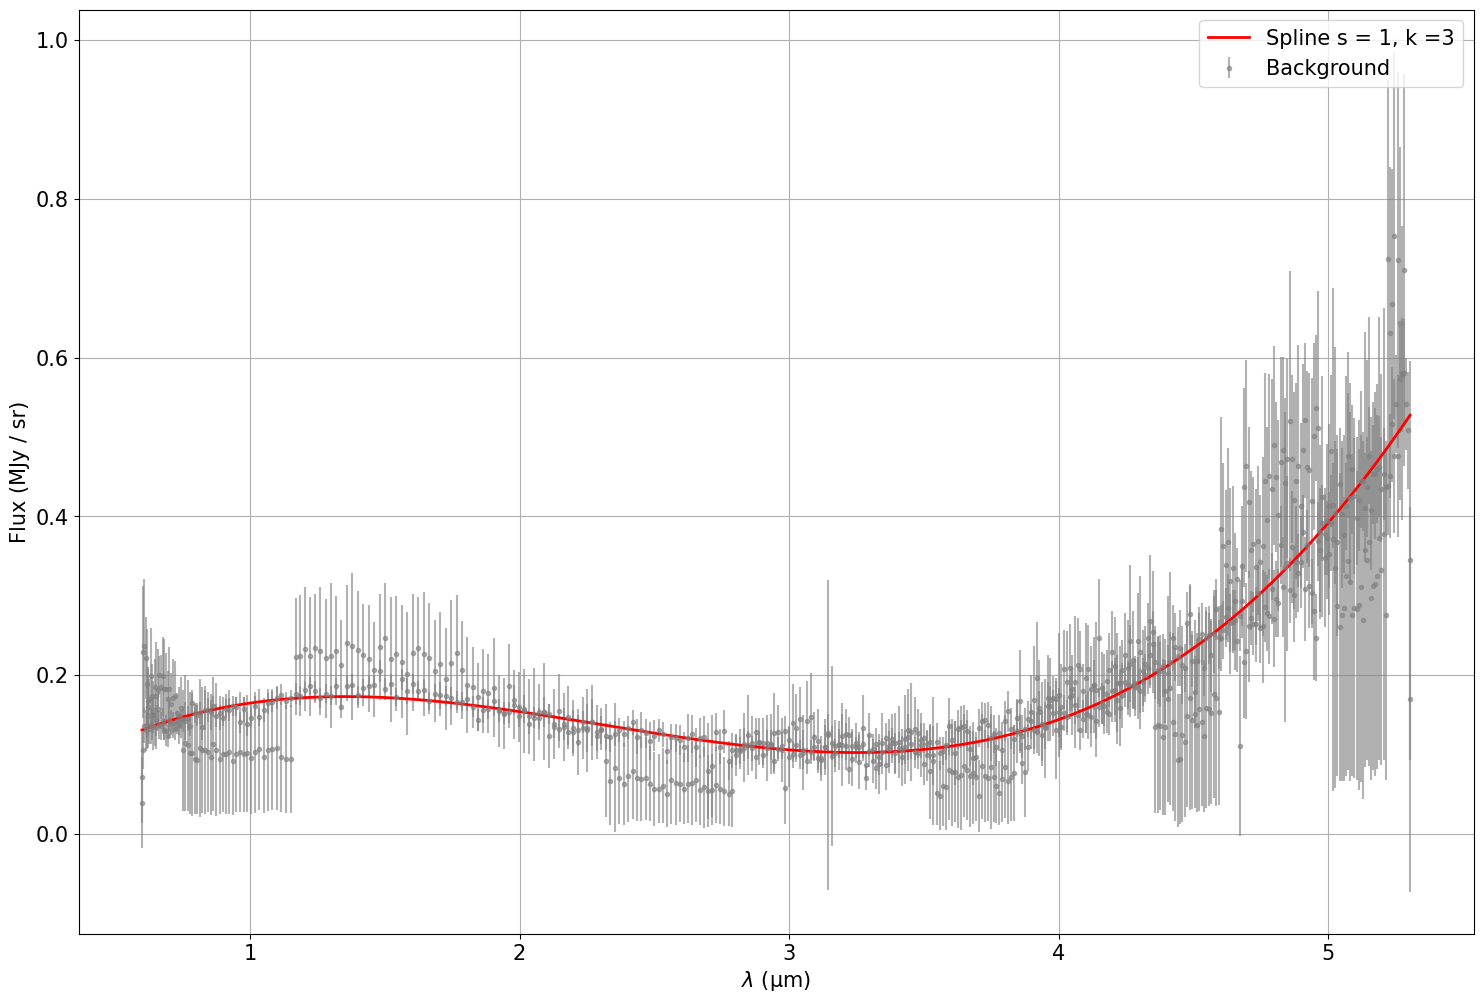
\includegraphics[scale=0.45]{assets/fit_spline.png}
  \caption{Extraction des spectres de fond sélectionnés sur la \figref{fig:extraction}, la spline ajustée est affichée en rouge. On remarque cependant que le nuage de points est séparé en 2 régimes, en raison du niveau de flux qui n'est pas le même sur une bande que sur l'autre.}
  \label{fig:spline_fit}
\end{figure}


\subsubsection{Aparté : Autres modèles d'ajustements}

Avant d'arriver au modèle actuel, plusieurs autres méthodes ont été envisagées et testées pour modéliser le fond.\\

Tout d'abord, les premiers tests ont été réalisés avant que l'étape de précalibration soit implémentée. Ceux-ci avaient donc lieu sur des images non traitées par un champ plat.

Une première méthode naïve consiste en l'extraction des bandes 2D de fond, le rejet des pixels au-dessus d'un certain seuil (garder les 50\% des plus lumineux, rejeter ceux au-dessus de 70\% de la valeur maximale...), puis l'interpolation de ces pixels rejetés à partir des pixels restants. L'interpolation pondérée de distance (\parencite{10.1145/800186.810616}) avait alors été choisie, en raison de son paramètre de puissance qui offrait un certain contrôle sur le degré de lissage de l'interpolation. L'allure générale du fond est en revanche perdue (\figref{fig:interpolation}).

L'interpolation utilisée est décrite dans l'équation \ref{eq:idw}, où $d_i = \sqrt{(x-x_i)^2 + (y-y_i)^2}$ avec $(x_i,y_i)$ la position d'un point à la valeur $z_i$ connue et $u$ le dégré de lissage.

\begin{equation}
  \label{eq:idw}
  f(x,y) = 
  \begin{cases}
    \frac{\sum_{i=0}^{N} d_i^{-u} \; \cdot z_i}{\sum_{i=0}^N \;d_i^{-u}} & d_i \neq 0 \; \forall i\\
    z_i & d_i = 0

  \end{cases}
\end{equation}

\begin{figure}[H]
  \centering
  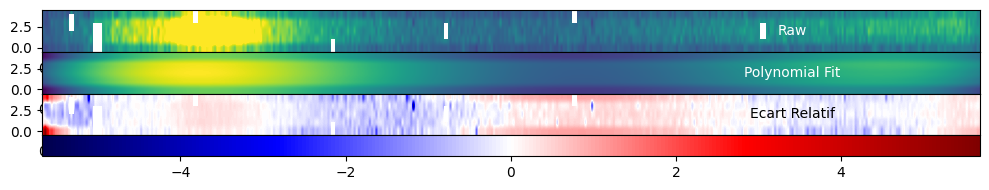
\includegraphics[scale=0.72]{assets/2D_polynomial.png}
  \caption{Comparaison entre données brutes d'une bande de fond (haut), un ajustement par un polynôme d'ordre 4 (milieu), et l'écart relatif $\frac{Raw - Fit}{Raw}$ (bas). Bien que l'allure générale semble suivie, des effets de bords importants sont visibles.}
  \label{fig:2D_polynomial}
\end{figure}

\begin{figure}[!h]
  \centering
     \begin{subfigure}[t]{0.45\textwidth}
        \centering
        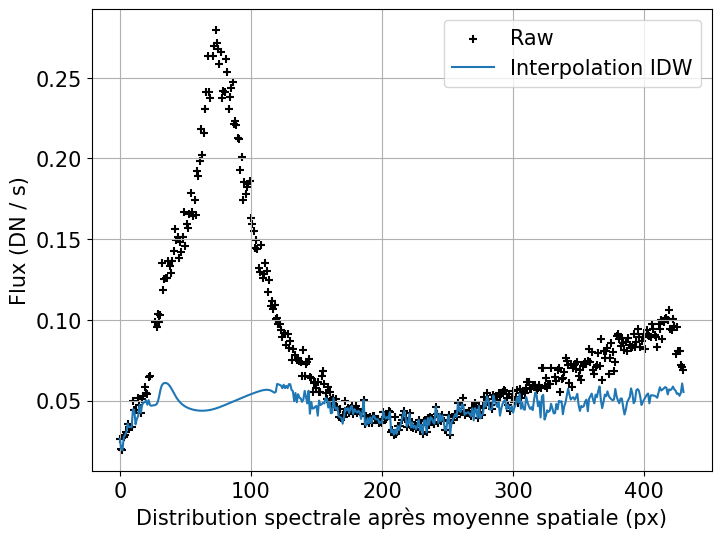
\includegraphics[scale=0.45]{assets/idw_interpolation.png}
        \caption{Moyenne spatiale du profil spectral d'une bande de fond, ainsi que d'une interpolation de ce même fond. On voit que les valeurs trop élevées sont tronquées, et que l'allure du profil n'est plus du tout suivie.}
        \label{fig:interpolation}
     \end{subfigure}
     \hfill
     \begin{subfigure}[t]{0.45\textwidth}
        \centering
        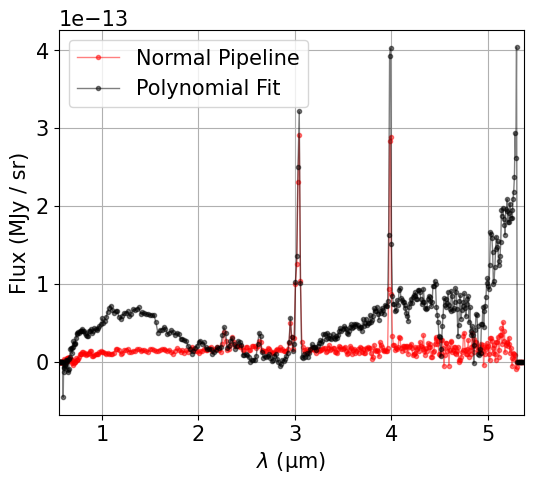
\includegraphics[scale=0.57]{assets/comparaison_normal_fit.png}
        \caption{Comparaison entre un spectre final obtenu par un traitement normal des données (rouge) et un spectre obtenu en ajustant le fond par des polynômes 2D}
        \label{fig:comparaison_fit_normal}
     \end{subfigure}
     \caption{}
\end{figure}

Une autre stratégie consiste en l'ajustement d'un polynôme en 2 dimensions sur chaque bande de fond. Cependant, malgré des premiers résultats prometteurs (\figref{fig:2D_polynomial}), les rapides variations sur les bords de l'image induisent des écarts importants avec les spectres obtenus par le traitement par défaut du pipeline (\figref{fig:comparaison_fit_normal}).\\

Enfin, en raison du manque de temps, certains détails ont dû être ignorés. L'algorithme actuel peut encore être amélioré, notamment sur la sélection des bandes de fond et sur l'ajustement de la spline. En effet, la méthode actuelle ne permet pas de propager les incertitudes sur l'ajustement aux données après la soustraction. De plus, il existe encore certains cas limites pour lesquels l'ajustement échoue, ou alors des cas où la spline peut être trouvée, mais celle-ci ne suit pas l'allure des données.


\subsubsection{Interpolation 2D et finitions}

Une fois notre spline $f(\lambda)$ obtenue, le spectre peut être interpolé en une image 2D à partir de la carte de longueurs d'ondes obtenue lors de la copie des données calibrées, à la fin de l'étape \texttt{Photom}. En effet, avant l'étape \texttt{ResampleSpec}, la direction de dispersion peut être légèrement déformée par rapport à l'axe horizontal. L'interpolation 2D a donc lieu avant cette étape afin de ne pas perdre d'informations lors du rééchantillonage inverse.

Les opérations mathématiques inverses de \texttt{Photom}, \texttt{BarShadow}, \texttt{PathLoss} et \texttt{FlatField} sont alors appliquées sur cette nouvelle image, donnant une image correspondant à une pseudo-observation du fond à travers les 3 fentes (\figref{fig:background}). Celle-ci est alors soustraite à l'image originale, donnant une image finale sur laquelle on applique les étapes suivantes du pipeline.

\begin{figure}[H]
  \centering
  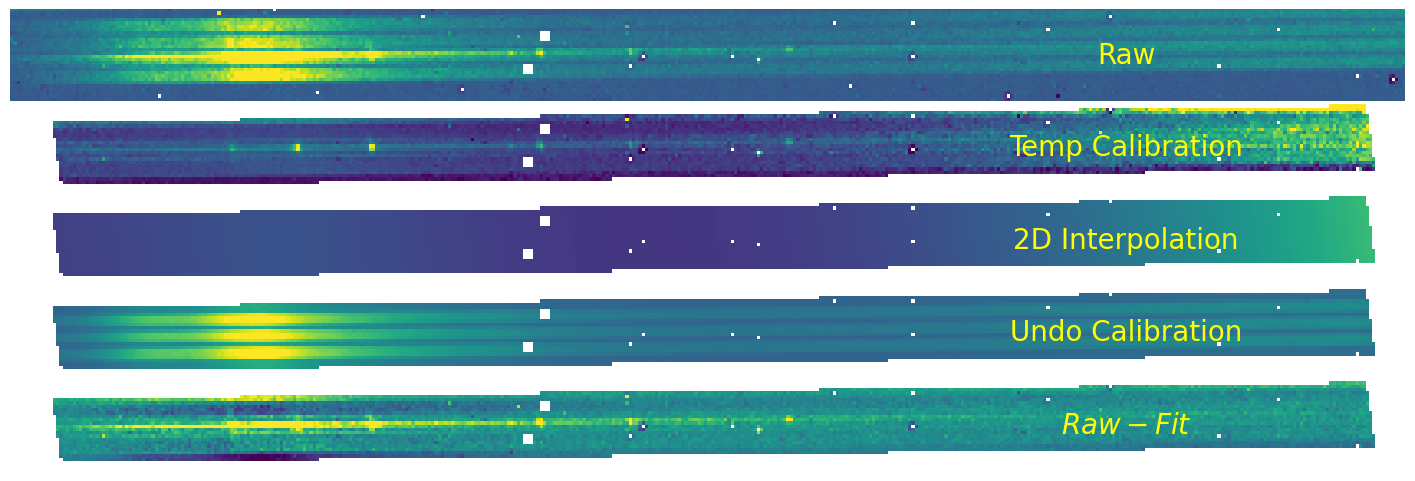
\includegraphics[scale=0.5]{assets/background_subtraction.png}
  \caption{Résumé des différentes opérations appliquées sur l'image d'une \textit{slitlet}. De haut en bas on a : l'image pré-algorithme, l'image temporairement calibrée, une nouvelle image formée par un ajustement du fond et une interpolation 2D, cette même image décalibrée, la soustraction de l'image originale par l'image du fond. Les bords manquants à l'image sont dus au traitement du \texttt{FlatField} qui ne calcule le champ plat qu'au niveau des 3 bandes. Ce qui est en dehors de cette zone est alors ignoré, même si un accidentel quatrième obturateur se trouve être ouvert comme ici.}
  \label{fig:background}
\end{figure}

\subsection{Résultats}

\begin{figure}[!h]
  \begin{subfigure}[t]{0.48\textwidth}
      \centering
      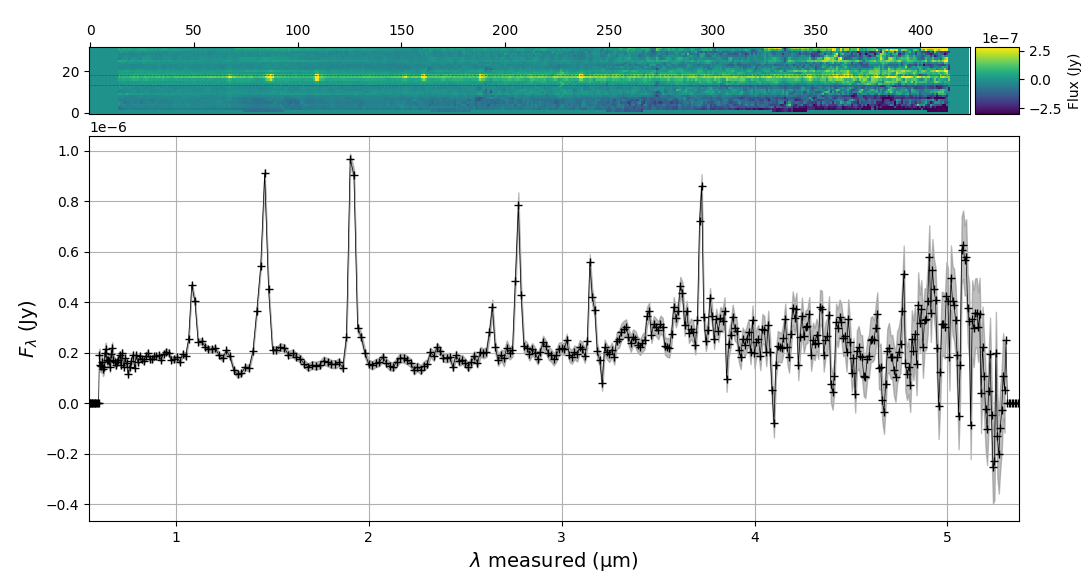
\includegraphics[width=1\textwidth]{assets/jw01345-o063_s32304_nirspec_clear-prism_extracted.png}
      \caption{Image en sortie du traitement du pipeline, ainsi qu'une extraction du spectre de l'objet principal. La bande extraite est sélectionnée à partir de la position supposée de la source dans l'image et mesure 7 pixels de haut.}
      \label{fig:extraction_32304}
  \end{subfigure}
  \hfill
  \begin{subfigure}[t]{0.48\textwidth}
      \centering
      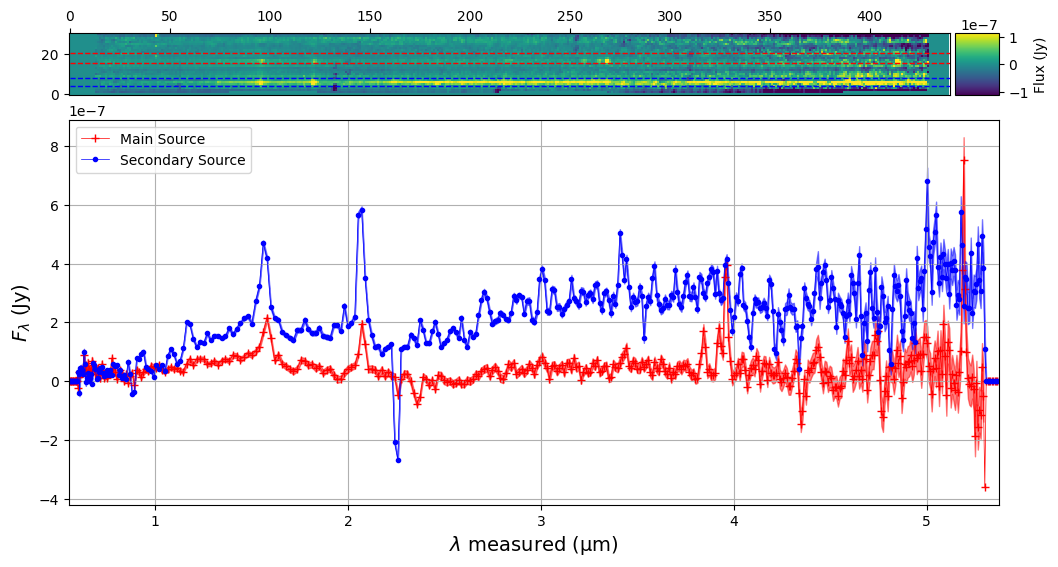
\includegraphics[width=1\textwidth]{assets/extraction_2_sources_P7-23642.png}
      \caption{Extractions d'une source principale (rouge) et d'une source secondaire (bleu)}
      \label{fig:extraction_2_sources}
  \end{subfigure}
  \caption{Extractions de quelques spectres obtenus par notre méthode}
\end{figure}

Une fois ce traitement effectué, on procède à une extraction des spectres des sources principales ainsi que des éventuelles sources secondaires. On affiche l'allure de ces spectres sur les \figref{fig:extraction_32304} pour le cas d'une source seule et \figref{fig:extraction_2_sources} pour le cas d'une source principale et une source secondaire.\\

On peut alors comparer les résultats obtenus par notre méthode personnalisée à ceux obtenus par le traitement classique. On réalise ceci sur la \figref{fig:comparaison_mast_custom}. On y observe clairement l'absence des traces négatives au-dessus et en dessous des raies sur l'image obtenue par notre traitement. Cependant, on remarque que le signal continu obtenu par la méthode classique semble légèrement plus important à certaines longueurs d'ondes que celui obtenu avec notre méthode. Ceci est par ailleurs confirmé en observant le dernier graphique, sur lequel est représenté le rapport signal sur bruit en fonction de la longueur d'onde. Seules les raies se retrouvent amplifiées par notre méthode.\\

\begin{figure}[!h]
  \centering
  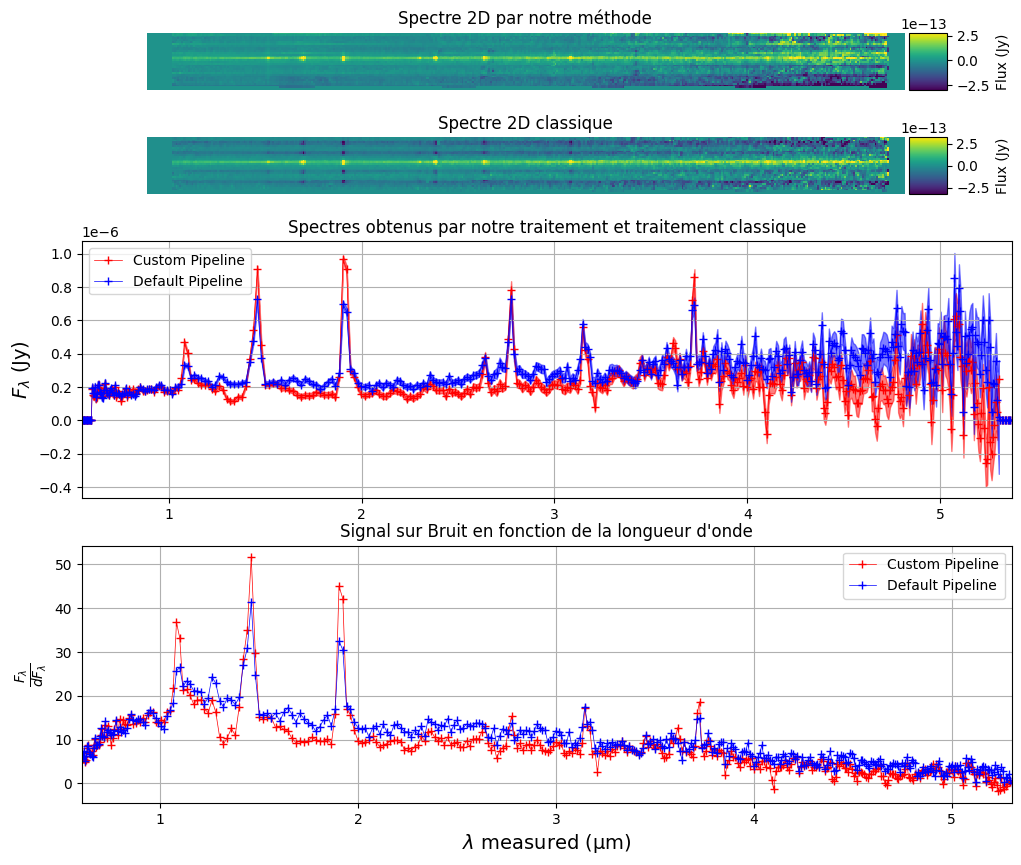
\includegraphics[scale=0.7]{assets/comparaison_spectres_mast_custom.png}
  \caption{Comparaison entre le traitement classique et notre traitement personnalisé. De haut en bas, on a : Le spectre 2D obtenu par notre méthode, le spectre 2D obtenu par la méthode classique, les spectres 1D extraits, avec en rouge notre méthode et en bleu la méthode classique, et le rapport signal sur bruit.}
  \label{fig:comparaison_mast_custom}
\end{figure}

\subsubsection{Simulation de données}

Pour tenter de comprendre ce résultat, nous avons essayé d'appliquer les 2 méthodes de soustraction (pixel par pixel et ajustement du fond) sur des données simulées.

Pour cela, on suppose un fond polynomial d'ordre 3, auquel on choisit les coefficients de manière à reproduire l'allure générale des signaux de fonds observés (à savoir un maximum local entre 1 et 2 microns, suivi d'une remontée vers $5 \mu m$).

\begin{equation}
  bkg(\lambda) = a \lambda^3 + b \lambda^2 + c \lambda + d \; , 
  \begin{cases}
    a = 0.04\\
    b = -0.3\\
    c = 0.7\\
    d = 0
  \end{cases}
\end{equation}

Le signal simulé d'une galaxie est constitué de 2 raies d'émissions au profil lorentzien (\ref{eq:lorentzien}) et d'une exponentielle en guise d'émission continue (\ref{eq:exponential}).

\begin{equation}
  \label{eq:lorentzien}
  \frac{A}{1 + (\frac{2(x-x_0)}{L})^2} \; ,
  \begin{cases}
   A = 5,3\\
   x_0 = 3.3, 1.8\\
   L = 0.06
  \end{cases}
\end{equation}

\begin{equation}
  \label{eq:exponential}
  A e^{x/T} - c \; ,
  \begin{cases}
   A = 1.2\\
   T = 6\\
   c = 0.5\\
  \end{cases}
\end{equation}


\begin{wrapfigure}{r}{8.5cm}
  \centering
  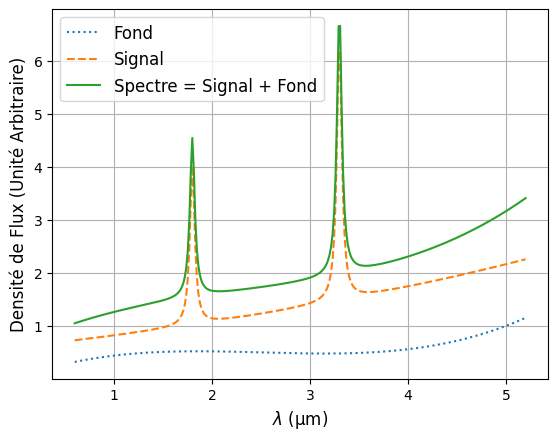
\includegraphics[scale=0.55]{assets/spectre_simulation.png}
  \caption{Allure du spectre simulé (vert), avec le fond polynomial (bleu) et le signal continu et 2 raies (orange)}
  \label{fig:simulated_spectrum}
\end{wrapfigure}

L'allure de ces spectres est représentée \figref{fig:simulated_spectrum}. Pour simuler l'apparence du spectre 2D, on étend verticalement la fonction représentant le fond, ainsi que celle représentant la source pour former 2 bandes de fond et une bande de signal (additionnée du fond). Ces 3 bandes sont alors permutées de façon à obtenir 3 observations, simulant le \textit{nodding} des vraies observations. Chaque bande est également multipliée par une gaussienne selon la direction verticale, centrée sur leur axe central, représentant les ombres résiduelles laissées par les bords des obturateurs. On ajoute finalement un bruit gaussien d'écart-type $\sigma = 0.1$. Les observations ainsi simulées sont visibles \figref{fig:simulated_observations}. On peut alors appliquer les algorithmes de soustraction afin de les comparer.

\begin{figure}[H]
  \centering
  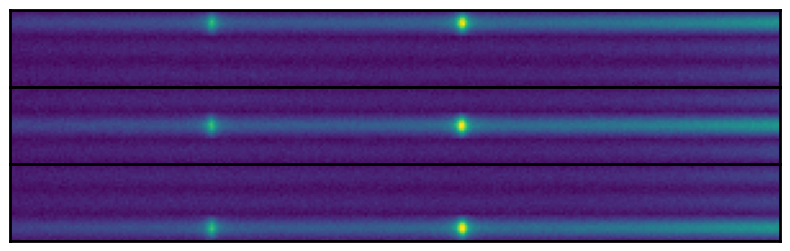
\includegraphics[scale=0.8]{assets/simulated_image.png}
  \caption{Simulation des 3 observations}
  \label{fig:simulated_observations}
\end{figure}

\begin{wrapfigure}{r}{8.5cm}
  \centering
  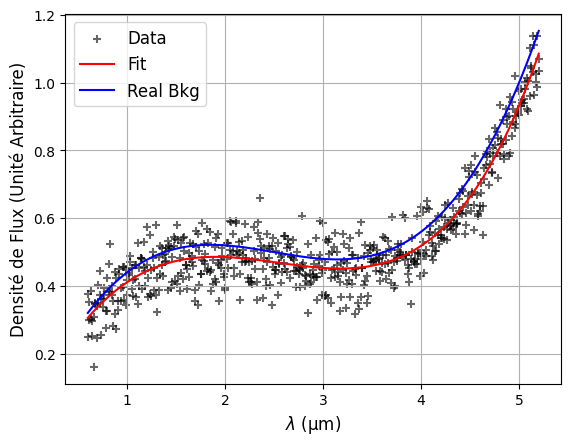
\includegraphics[scale=0.55]{assets/fit_simulated.png}
  \caption{Ajustement d'une spline (rouge) sur les données simulées (points noirs) par rapport au modèle de fond connu (bleu)}
  \label{fig:simulated_fit}
\end{wrapfigure}

En ajustant la spline au fond, on remarque \figref{fig:simulated_fit} une légère sous-estimation de son allure, en raison de la fenêtre gaussienne résiduelle qui vient abaisser les valeurs des pixels sur les bords de chaque bande. Pour s'affranchir de cet effet, on pourrait alors réduire la hauteur de la fenêtre d'extraction, mais cela aurait pour conséquence de diminuer le nombre de points et de potentiellement biaiser l'ajustement, qui serait, en effet, plus susceptible au bruit.\\

On trace alors les extractions obtenues selon les méthodes de soustraction \figref{fig:comparaison_simulated}, que l'on remarque être relativement similaire. En traçant l'écart relatif au carré $(\frac{extract - signal}{signal})^2$ (moyenné sur des intervalles de longueur $0.1 \mu m$), on voit par ailleurs que les résultats obtenus sont comparables pour les 2 méthodes, avec une légère préférence pour la méthode classique (pixel par pixel), puisque la méthode par ajustement du fond sous-estime ce dernier, comme discuté plus haut.

Cependant, en modifiant légèrement les bandes de fond de façon à simuler l'allure d'une source étendue visible à travers plusieurs obturateurs (à chaque bande de fond est ajouté le spectre simulé de la source, multiplié par un coefficient $c=0.05$), on observe une nette amélioration de la méthode par ajustement par rapport à la méthode classique (\figref{fig:comparaison_simulated_extended}).\\

Ainsi, comme attendu, notre méthode est plus efficace dans la soustraction du fond dans le cas d'une source étendue. Ce résultat sur les données simulées ne semble cependant pas se refléter sur les données réelles. Une explication possible est une combinaison entre la sous-estimation liée aux pertes de lumière résiduelles sur les bords d'une bande et une surestimation due à l'éventuelle présence du spectre d'une source étendue dans les bandes de fond. En raison du manque de temps, nous ne pourrons pas explorer ces pistes plus en détails dans le cadre de ce stage.

\begin{figure}[H]
  \centering
  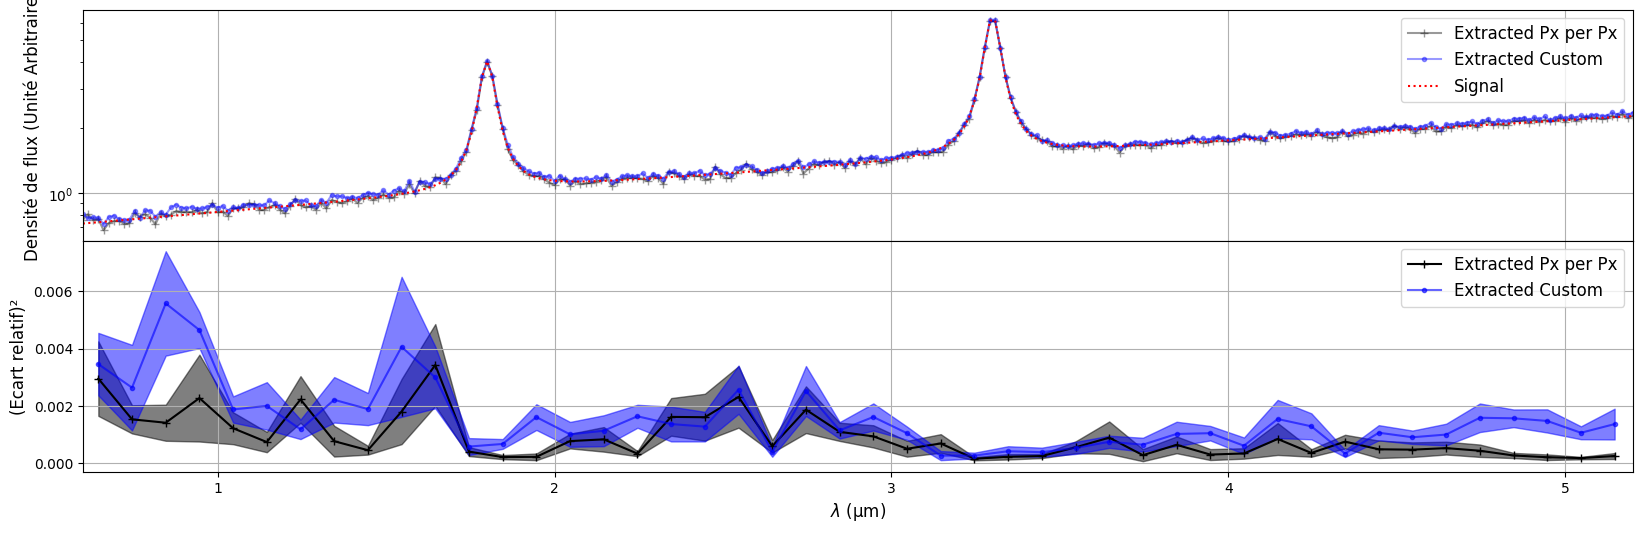
\includegraphics[scale=0.4]{assets/comparaison_simulated.png}
  \caption{Comparaison entre les 2 méthodes de soustraction du fond sur données simulées. En haut, le spectre extrait après méthode classique (noir) et méthode par ajustement du fond (bleu), ainsi que l'allure réelle du signal (rouge). En bas, l'écart relatif au carré $(\frac{extract - signal}{signal})^2$ montre que les 2 extractions sont comparables, bien que légèrement en faveur de l'extraction pixel par pixel}
  \label{fig:comparaison_simulated}
\end{figure}

\begin{figure}[H]
  \centering
  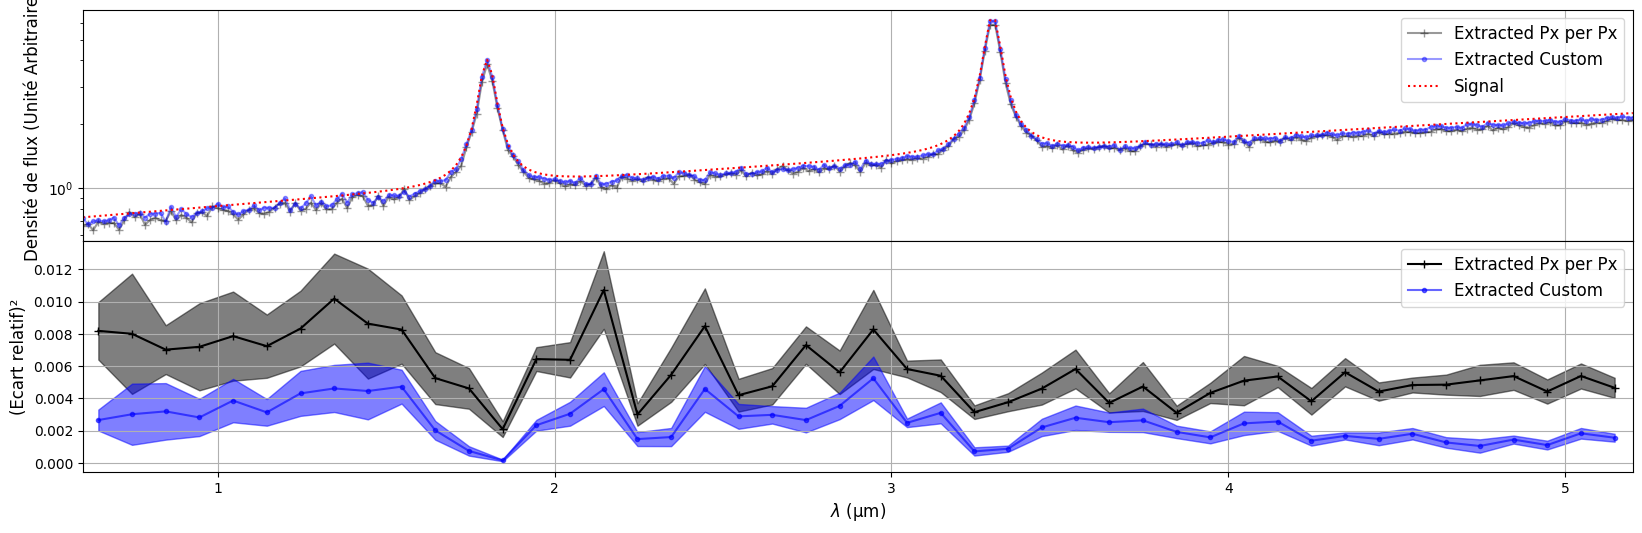
\includegraphics[scale=0.4]{assets/comparaison_simulated_extended.png}
  \caption{Comparaison entre les 2 méthodes sur données simulées avec source étendue (5\% du signal est ajouté au fond). On remarque qu'ici l'écart relatif est largement en faveur de notre extraction.}
  \label{fig:comparaison_simulated_extended}
\end{figure}


\section{Analyse des spectres}

\subsection{Présentation de CIGALE}

\glsreset{cigale}
\gls{cigale} \parencite{cigale} est un outil permettant de modéliser l'émission d'une galaxie, ses raies d'émissions, son absorption par la poussière, son spectre continu, son \textit{redshift}, de comparer ces modèles aux données afin d'établir le plus vraisemblable et ainsi de déterminer les paramètres physiques, chimiques et cosmologiques des galaxies observées.

Les données utilisées avec \gls{cigale} sont d'ordinaire des données photométriques obtenues dans différentes bandes du spectre électromagnétique, des rayons X à la radio. Cependant, nous travaillons ici sur une version en accès anticipé de l'outil nous donnant la possibilité d'étudier des données spectroscopiques.\\

La génération d'un modèle se base sur une série d'étapes successives (on ignore ici les étapes liées aux noyaux actifs de galaxies, car nous partons de l'hypothèse d'une émission majoritairement due à la formation stellaire) :

\begin{itemize}
  \item[1.] Calcul de l'histoire de formation stellaire, ou \gls{sfh}
  \begin{itemize}
    \item Module \texttt{sfhdelayed} : On modélise un \textit{"burst"} de formation d'étoiles ainsi :
    
     $SFR(t) \propto \frac{t}{\tau^2} \cdot e^{-t/\tau}$, avec $\tau$ le temps au maximum de formation stellaire (en supposant le temps $t=0$ comme le début du \textit{burst}).

    La \gls{sfr} en fonction du temps est d'abord caractérisée par un premier burst, impliquant en général la majorité de la formation d'étoiles, suivie plus tard d'un autre \textit{burst}.
  \end{itemize}

  \item[2.] Détermination du spectre stellaire à partir de la \gls{sfh}
  \begin{itemize}
    \item Module \texttt{bc03} : Modélise la fonction de masse initiale (\gls{imf}), c'est-à-dire la densité de probabilité qu'une étoile ait une certaine masse lors de la formation stellaire. Le module modélise alors l'émission individuelle des étoiles selon leur masse et leur métallicité. On utilise ici la distribution données par \cite{2003PASP..115..763C}.
  \end{itemize}

  \item[3.] Calcul de l'émission nébulaire, notamment des raies d'émission
  \begin{itemize}
    \item Module \texttt{nebular} : Simule l'émission du gaz ionisé par le rayonnement des étoiles massives (continue et raies) en prenant en compte la metallicité $Z$ de celui-ci, la densité électronique $N_e$, le degré d'ionisation adimensionné $U$ (variant de $10^{-4}$ à $10^{-1}$) (le rapport entre la densité de photons ionisant sur la densité d'atomes d'hydrogène \parencite{Astrophysics-of-the-Diffuse-Universe}).
  \end{itemize}

  \item[4.] Calcul de l'absorption ultraviolette par la poussière
  \begin{itemize}
    \item Module \texttt{dustatt\_modified\_starburst} : Décrit l'extinction UV $E_{B-V}$ comme une loi de puissance, accompagnée d'un pic lorentzien correspondant à un "\textit{UV bump}" empirique, présent dans le spectre de la plupart des galaxies proches \parencite{10.1093/mnras/stac1313}. Cette extinction peut être définie différemment pour les étoiles vieilles et les étoiles jeunes.
  \end{itemize}

  \item[5.] Calcul de la réémission des poussières dans l'infrarouge
  \begin{itemize}
    \item Module \texttt{dl2014} : Le principe fondamental derrière \gls{cigale} est la conservation de l'énergie. Les photons absorbés par la poussière en ultraviolet sont réémis en infrarouge moyen et lointain. Ce module simule l'émission de cette poussière (silicates, hydrocarbures, etc) en 2 parties : l'émission diffuse liée au chauffage par les étoiles et l'émission par chauffage dans les zones de formation stellaire, décrite par une loi de puissance. Cependant, ces émissions ne se situent pas dans l'intervalle de longueurs d'ondes observé par \gls{nirspec}, aux \textit{redshifts} souhaités. Leur influence sera donc négligeable sur les spectres observés et ces paramètres seront alors très peu contraints.
    
  \end{itemize}
  \item[6.] Décalage par redshift
  \begin{itemize}
    \item Module \texttt{redshifting} : Le spectre réalisé jusqu'à présent est celui dans le référentiel au repos de la galaxie. Ce module permet de passer au référentiel observé en appliquant un \textit{redshift}. On a comme nouvelles longueurs d'ondes $\lambda' = \lambda \cdot (1+z)$ et comme nouveau flux $F_\lambda' = F_\lambda / (1+z)$. Est également calculé l'absorption par le milieu intergalactique.
  
  \end{itemize}
\end{itemize}

\begin{wrapfigure}{r}{7cm}
  \centering
  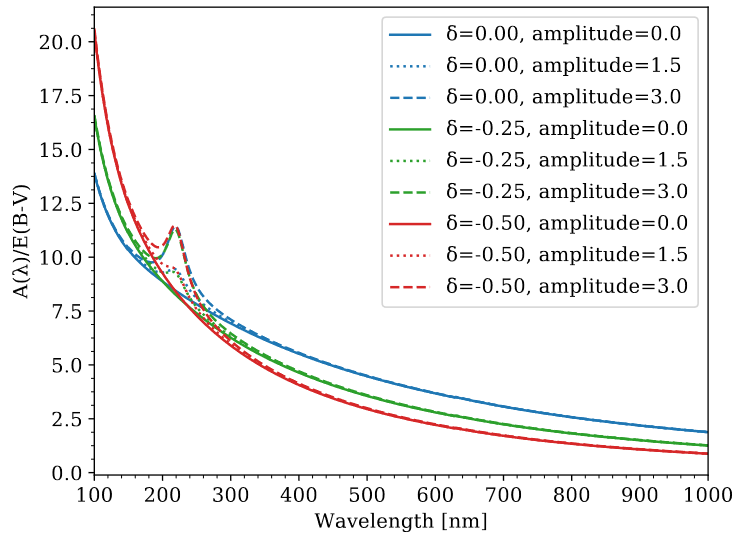
\includegraphics[scale=0.5]{assets/absorption_uv.PNG}
  \caption{Courbes d'atténuations, avec \textit{l'UV bump} clairement visible pour différentes amplitudes. $\delta$ est le coefficient de la loi de puissance. \customcite{cigale}}
\end{wrapfigure}

Etant donné le nombre important de paramètres pris en compte dans un modèle donné, \gls{cigale} a recours à une grille de valeurs prédéfinies par l'utilisateur. Contrairement aux méthodes habituelles d'ajustement à grand nombre de paramètres, telle que la descente de gradient ou la méthode de Monte-Carlo par chaines de Markov, l'approche grille permet de fortement réduire le nombre de modèles à calculer, puisqu'un seul modèle peut être utilisé plusieurs fois pour chaque spectre.

\gls{cigale} va donc calculer les différents modèles $m_i$ à partir des paramètres donnés en entrée des modules et déterminer le $\chi^2 = \sum_{i} (\frac{f_i - \alpha \cdot m_i}{\sigma_i})^2$ avec les données $f_i$ et leur incertitude $\sigma_i$ ($\alpha$ est ici un facteur de normalisation du spectre, le véritable $\chi^2$ est par ailleurs décrit en détail dans l'article de présentation de \gls{cigale} \parencite{cigale}). Pour chaque $\chi^2$ est alors calculé la vraisemblance $\propto e^{-\chi^2 / 2}$, ce qui permet alors, au maximum de vraisemblance, de déterminer les paramètres les plus adaptés ainsi que leur incertitude à partir de l'écart-type du pic.\\

On procède donc en 2 étapes. La première consiste en une analyse approximative et rapide des 616 spectres, dont 24 sources secondaires, dans le but d'obtenir une estimation de leur \textit{redshift} $z$. Une fois celui-ci obtenu, chaque spectre se retrouve associé à un \textit{redshift}, nous permettant ainsi de découpler les phases "mesure du \textit{redshift}" et "mesure des autres paramètres". Le fichier \texttt{pcigale.ini} contenant la liste des paramètres et leurs valeurs utilisées lors du calcul des modèles est donnée en annexe \ref{pcigale.ini}.

\subsubsection{Résultats généraux}

On affiche ici quelques modèles en sortie de \gls{cigale} (\figref{fig:P5_s32304_best_model} et \figref{fig:P7_s23642_best_models}).

Concernant la \figref{fig:P7_s23642_best_models}, bien que les allures des spectres ne sont pas exactement identiques, le redshift est identique entre les 2 sources. Ceci est cohérent avec la présence des mêmes raies sur leurs spectres respéctifs. Celà laisserait penser qu'il s'agit de la même source étendue, cependant, il est alors peu clair pourquoi la bande entre les 2 sources ne présente pas une allure similaire.

\begin{figure}[!h]
  \centering
  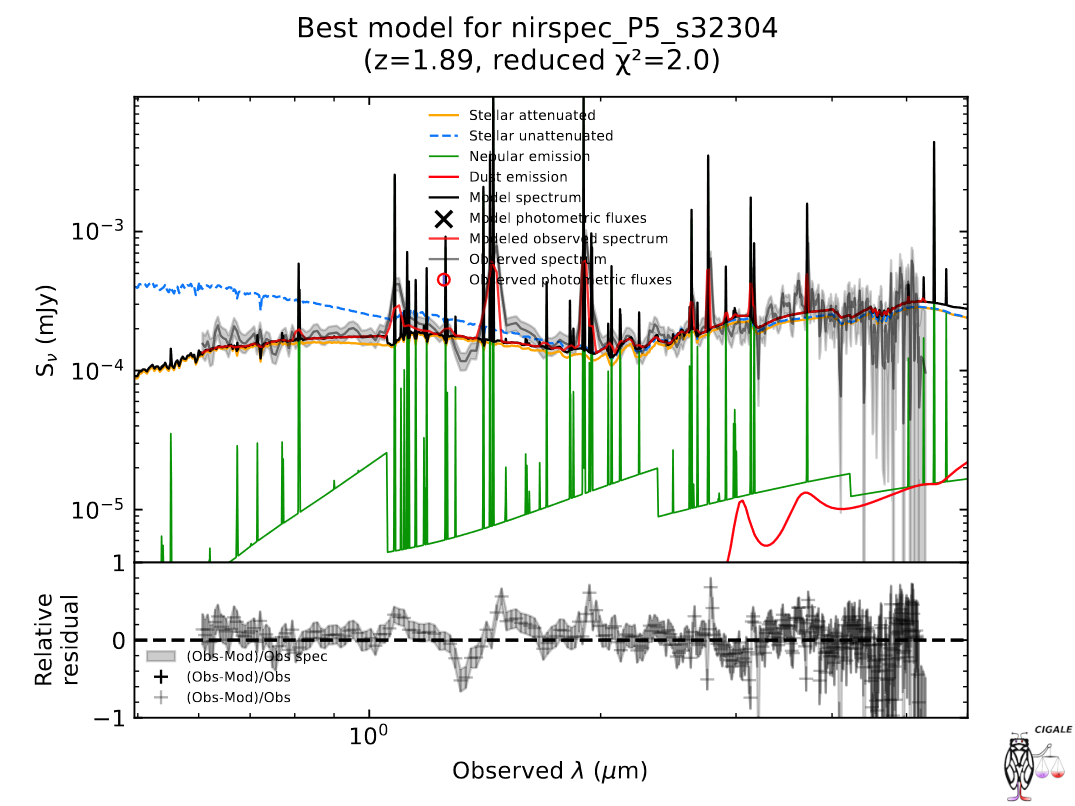
\includegraphics[width=\textwidth]{assets/nirspec_P5_s32304_best_model.png}
  \caption{Meilleur modèle trouvé par \gls{cigale} pour notre spectre d'illustration \figref{fig:extraction_32304}. Les différentes composantes du spectre sont affichées de différentes couleurs dans le graphique supérieur, en particulier les données en gris et le spectre prédit par le modèle en rouge. Le graphique du bas affiche l'écart relatif entre ces 2 courbes.}
  \label{fig:P5_s32304_best_model}
\end{figure}

\begin{figure}[!h]
  \centering
     \begin{subfigure}[t]{0.45\textwidth}
         \centering
         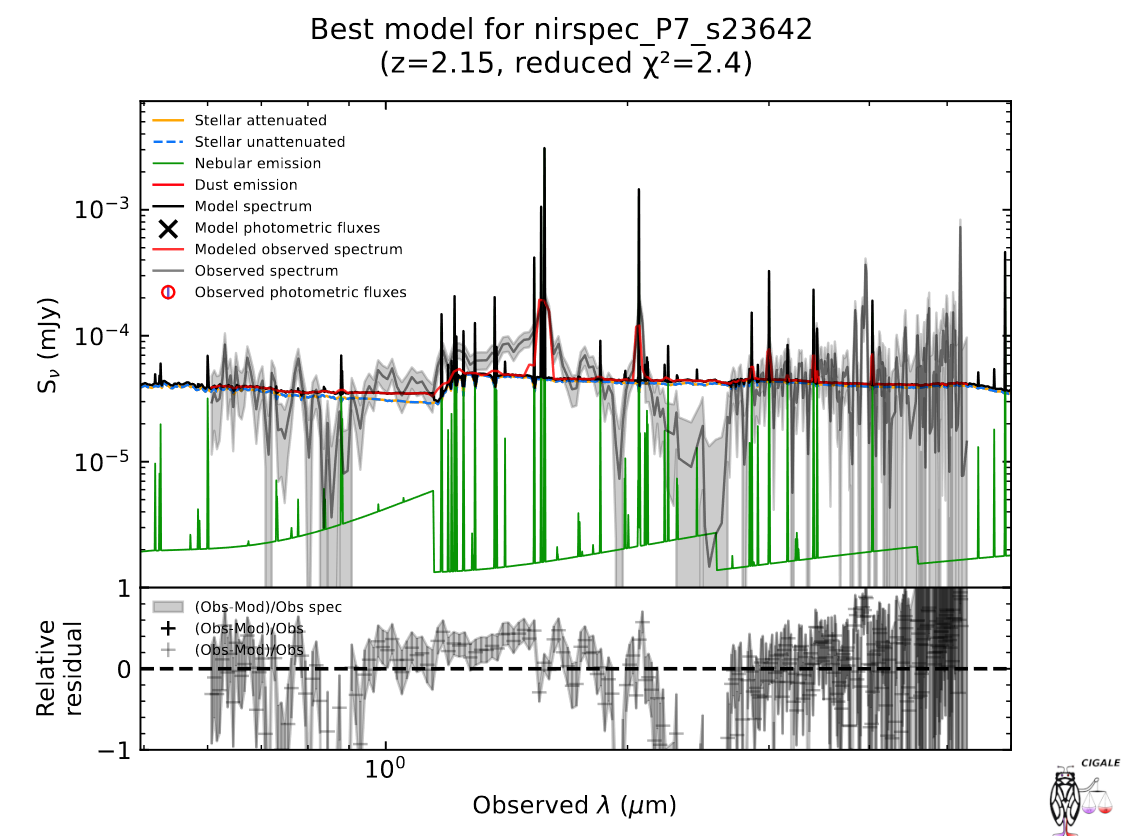
\includegraphics[width=1.3\textwidth]{assets/nirspec_P7_s23642_best_model.png}
         \caption{Meilleur modèle pour la source principale de la \figref{fig:extraction_2_sources}.}
     \end{subfigure}
     \hfill
     \begin{subfigure}[t]{0.45\textwidth}
         \centering
         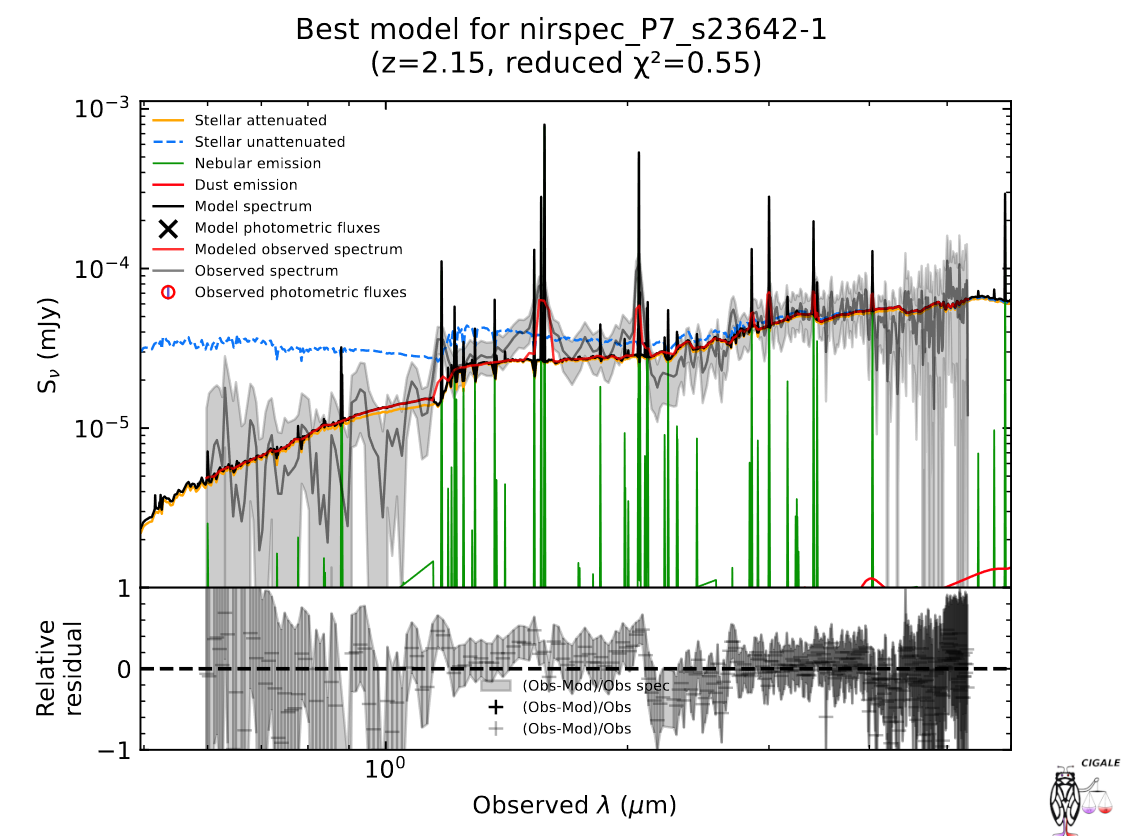
\includegraphics[width=1.3\textwidth]{assets/nirspec_P7_s23642-1_best_model.png}
         \caption{Meilleur modèle pour la source secondaire de la \figref{fig:extraction_2_sources}.}
     \end{subfigure}
     \caption{}
     \label{fig:P7_s23642_best_models}
\end{figure}

\subsubsection{Discussion sur le redshift}

\begin{figure}[!h]
  \centering
  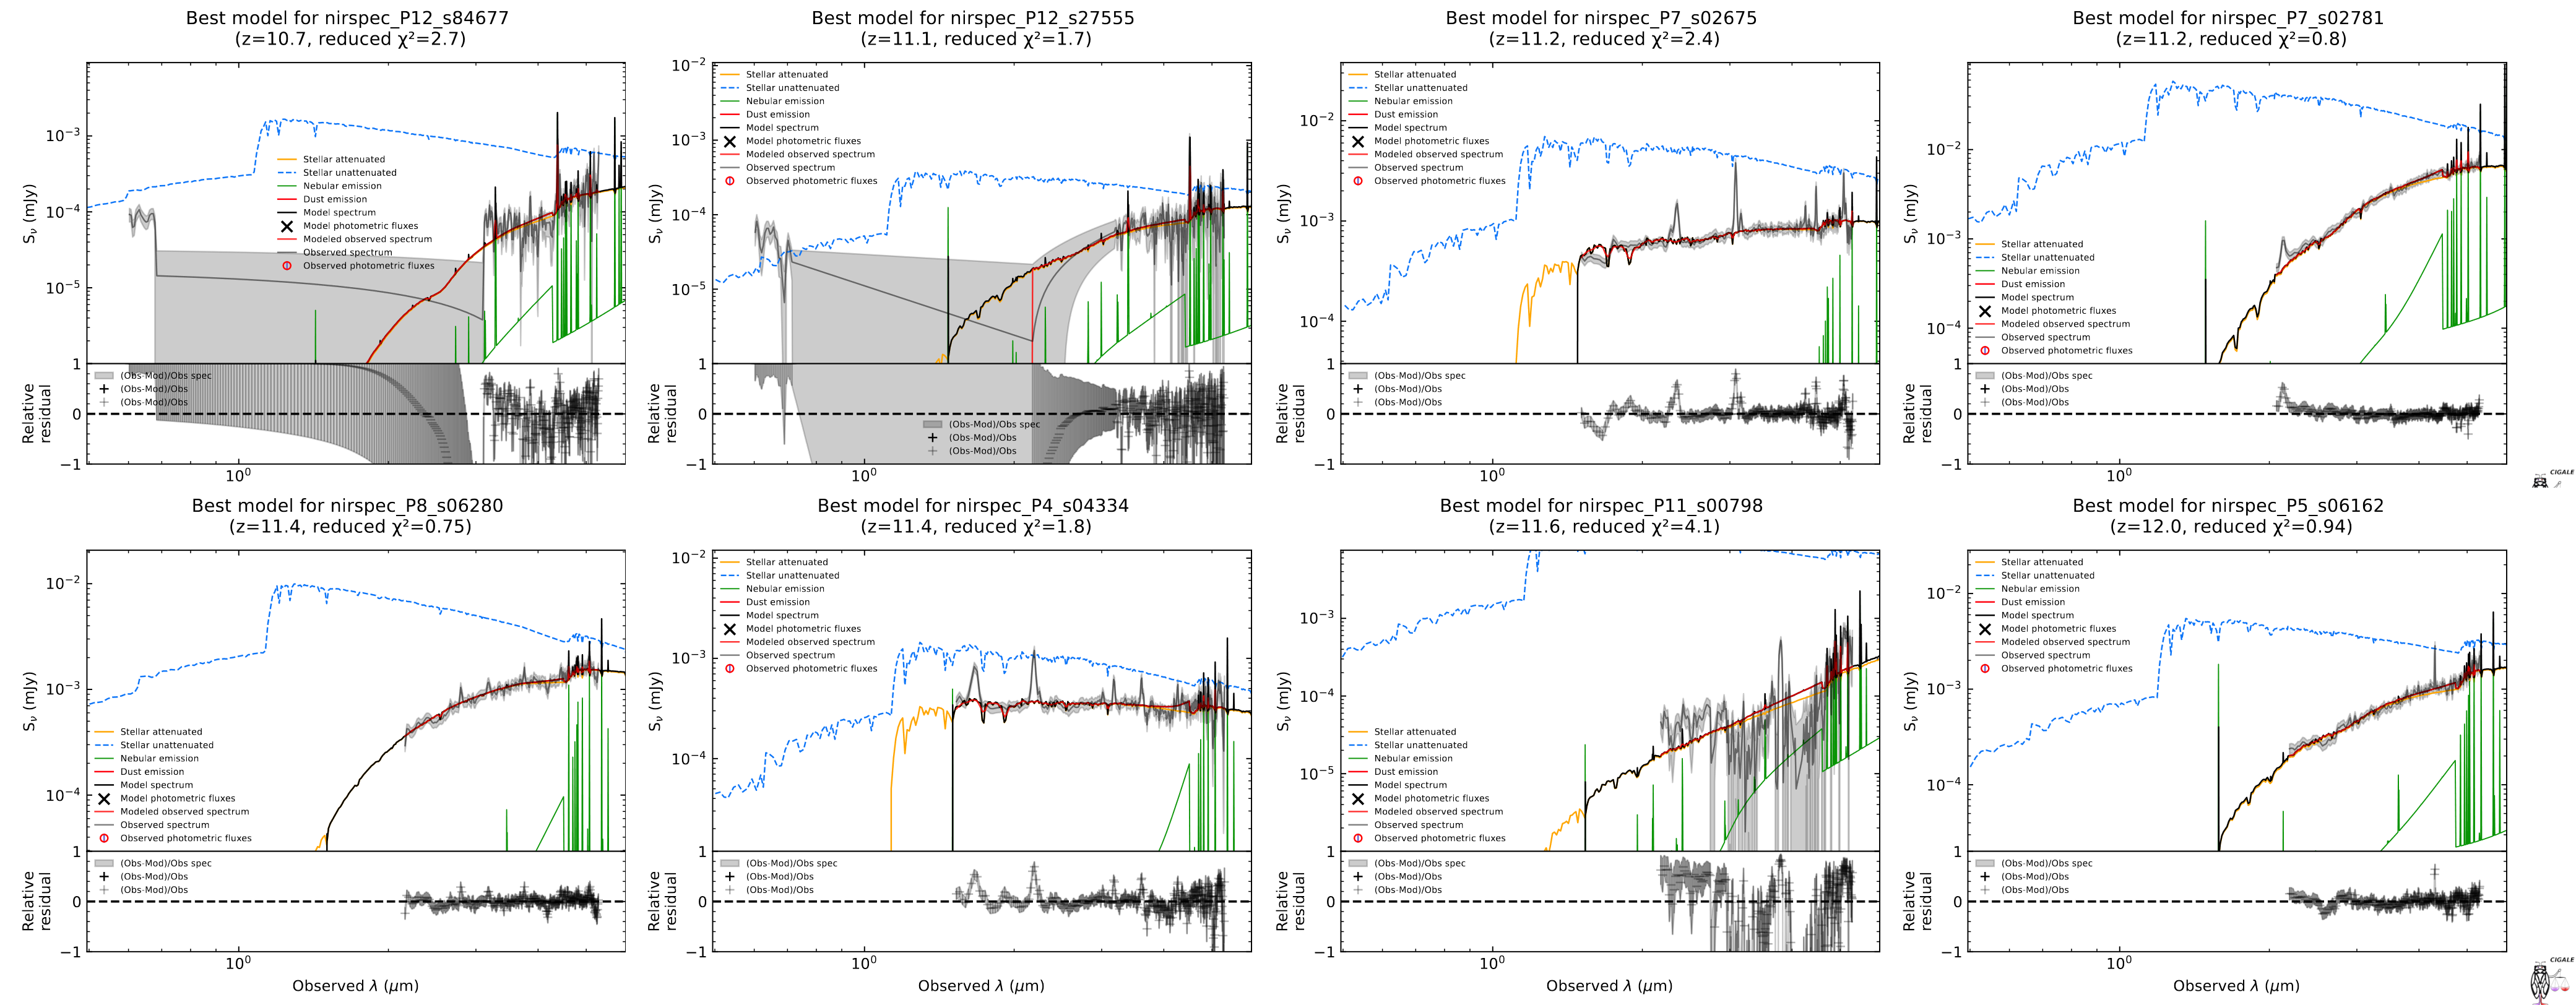
\includegraphics[width=1.1\textwidth]{assets/high_redshift_models.png}
  \caption{Spectres des 8 galaxies supposément à $z > 9$}
  \label{fig:high_redshift}
\end{figure}

Parmi les 515 galaxies pour lesquelles un ajustement a été trouvé, 8 d'entre elles ont à priori un \textit{redshift} supérieur à 9 (voir \figref{fig:high_redshift}), variant de 10.7 à 11.6. Nous avons cependant plusieurs raisons de penser que ces valeurs sont inexactes.

\begin{figure}[!h]
  \centering
  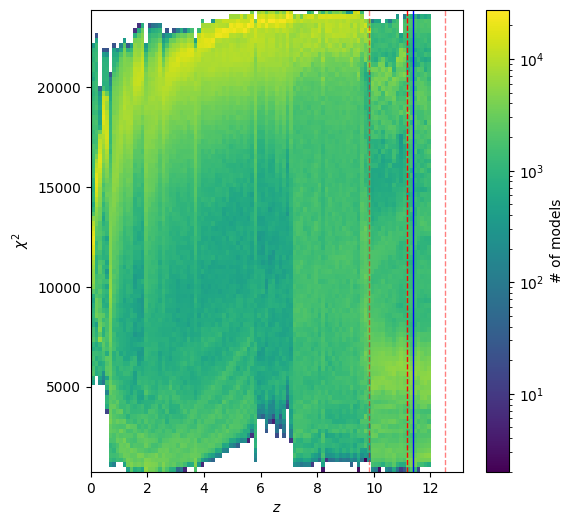
\includegraphics[scale=0.5]{assets/chi2_high_redshift.png}
  \caption{Représentation de la distribution du nombre de modèles générés en fonction de leur $\chi^2$ et du \textit{redshift} $z$. On trace en rouge la valeur de $z$ de la source P7-2675 déterminée à partir de distribution des $\chi^2$, accompagnée de son incertitude indiquée par les traits rouges continus. On trace en bleu la valeur de $z$ uniquement sélectionnée à partir de la grille de paramètres d'entrée.}
  \label{fig:chi2}
\end{figure}

Premièrement, les \textit{redshift} observés ne coïncident pas avec les objets à $z > 9$ observés par \gls{ceers} (\cite{2024ApJ...969L...2F}, \cite{ceers_high_redshift}).

Deuxièmement, bien que le continu semble correctement ajusté pour certains de ces spectres, l'absence flagrante de raies sur les modèles, là où elles sont pourtant présentes sur les données, est un autre indicateur de la mauvaise estimation de $z$.

Enfin, on peut choisir d'étudier le $\chi^2$ des modèles en fonction du \textit{redshift}. On réalise ceci dans la \figref{fig:chi2}, où l'on représente également le nombre de modèles correspondants aux couples $(z,\chi^2)$. En s'intéressant aux valeurs minimales des $\chi^2$ en fonction de $z$, on remarque que le \textit{redshift} trouvé n'est pas l'unique minimum local des $\chi^2$. On peut en effet en identifier un autre aux alentours de $z \approx 2$.

Pour toutes ces raison, nous allons par la suite ignorer les objets marqués comme étant à $z > 9$.

\subsubsection{Étude des doubles sources}

Après élimination des sources doubles pour lesquelles les ajustements ont échoué, on s'intéresse à 3 spectres 2D : \figref{fig:P4_s19960}, \figref{fig:P5_s14754} et \figref{fig:P7_s02962}.

\begin{figure}[!h]
  \centering
  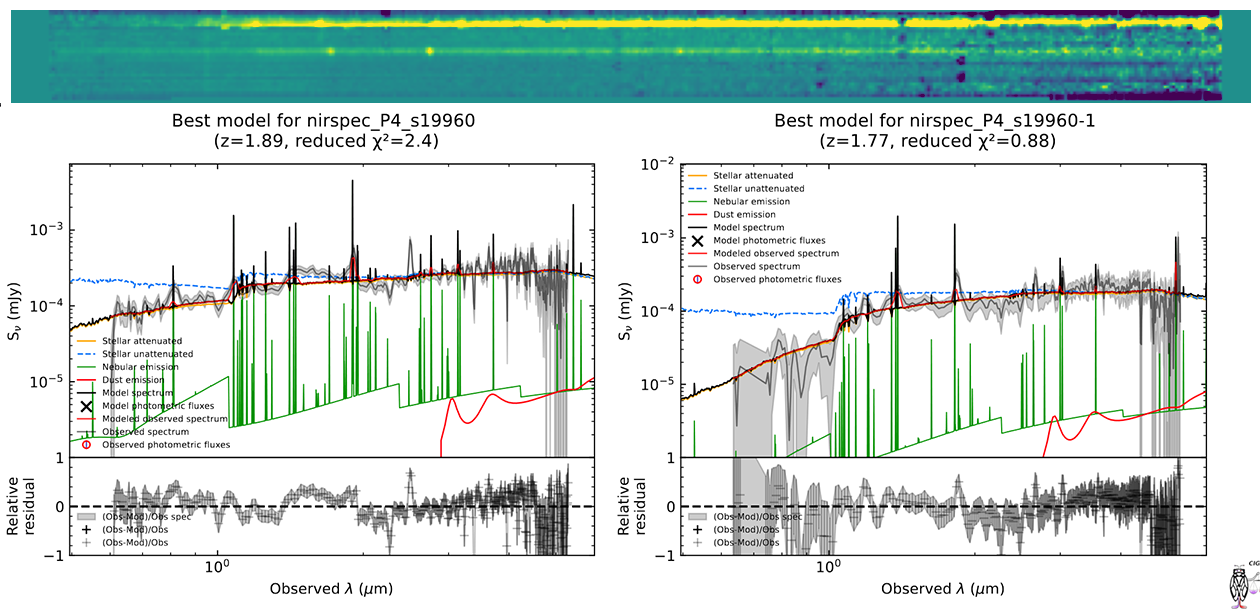
\includegraphics[width=1\textwidth]{assets/double_P4_s19960.png}
  \caption{Spectre 2D des 2 sources (haut), avec ajustement d'un modèle sur le spectre principal (gauche) et le spectre secondaire (droite). L'allure similaire des modèles ainsi que le redshift quasi-identique laisse à penser qu'il s'agirait de la même source, étendue dans le champ de plusieurs obturateurs. Cependant, en supposant les ajustements corrects, le \textit{redshift} devrait être précis à $0.01$ près. Il est donc plus probable qu'il s'agisse de 2 galaxies visuellement proches mais séparées de $68 Mpc$.}
  \label{fig:P4_s19960}
\end{figure}

\begin{figure}[!h]
  \centering
  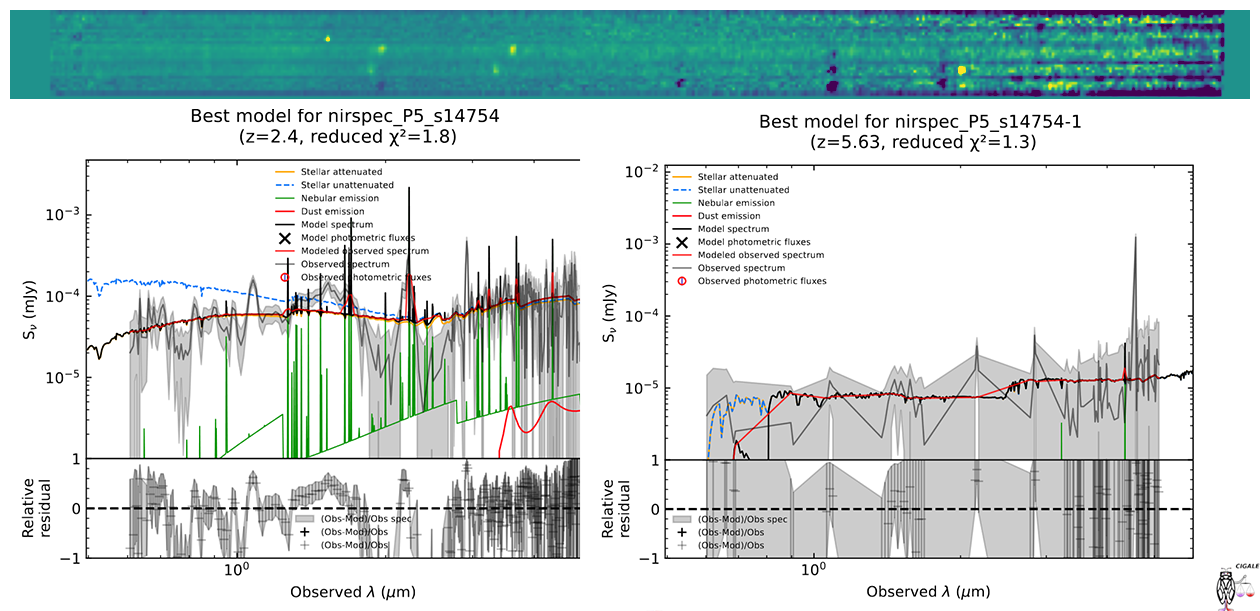
\includegraphics[width=1\textwidth]{assets/double_P5_s14754.png}
  \caption{Les 2 spectres semblent visuellement similaires sur l'image du haut. Cependant, les ajustements ne semblent pas suivre leur allure, en particulier pour le spectre secondaire, où le rapport signal sur bruit trop faible de certains points leur vaut d'être ignoré par l'ajustement.}
  \label{fig:P5_s14754}
\end{figure}

\begin{figure}[!h]
  \centering
  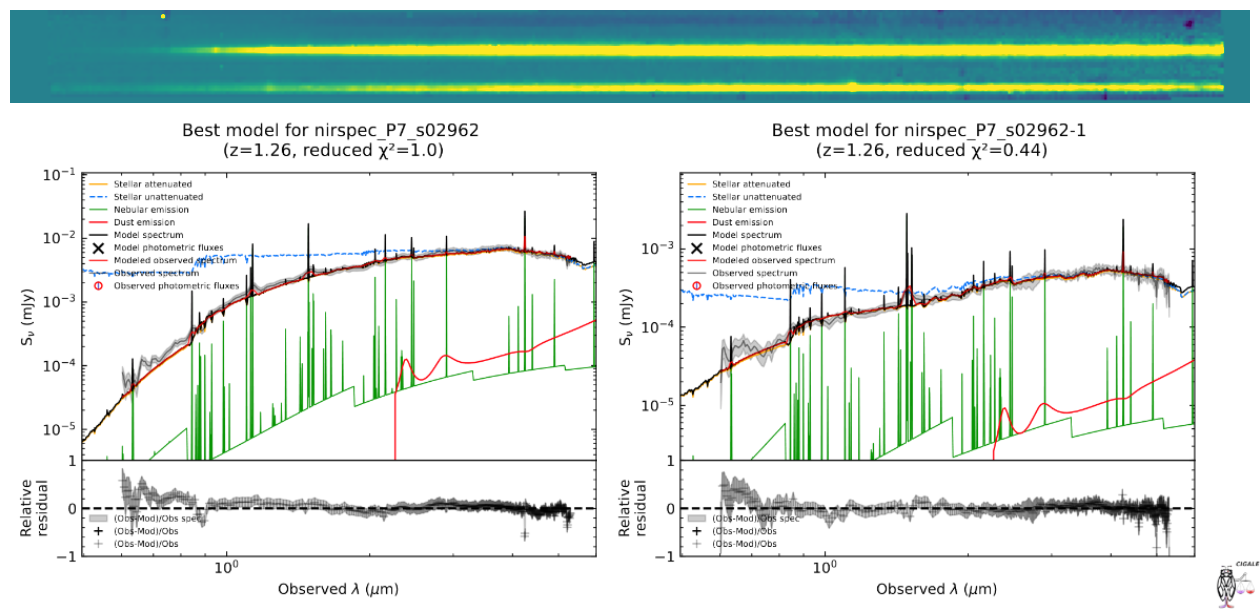
\includegraphics[width=1\textwidth]{assets/double_P7_s02962.png}
  \caption{À nouveau, les ajustements semblent relativement similaires, de même redshift, tendant à montrer qu'il s'agit probablement à nouveau d'une source étendue. Il n'est néanmoins pas clair pourquoi, à nouveau, la bande entre les 2 spectres ne présente pas une allure similaire. Il pourrait s'agir de 2 galaxies dans un même amas, donc au même \textit{redshift}.}
  \label{fig:P7_s02962}
\end{figure}

\subsubsection{Étude des paramètres déduits}

Notre sélection de galaxies désormais modélisée, il devient possible d'extraire les paramètres servant à construire le meilleur ajustement, mais également d'estimer ceux-ci à partir du $\chi^2$, permettant donc de s'affranchir de la discrétisation de l'approche grille.\\

Un premier résultat à vérifier est l'évolution de la séquence principale galactique avec le redshift. En effet, il existe une relation empirique entre le taux de formation stellaire et la masse stellaire d'une galaxie \parencite{2007ApJ...660L..43N}. Cette séquence principale peut, en première approche, être approximée par une loi de puissance. En traçant le diagramme log-log de la \gls{sfr} en fonction de $M_*$, on s'attend donc à observer une droite, ce qui est effectivement le comportement retrouvé \figref{fig:main_sequence}. On remarque que le comportement de cette séquence principale varie bien avec le redshift \parencite{10.1093_mnras_stac3214} et on trace donc les coefficients directeurs et ordonnées à l'orgine en fonction du redshift (\figref{fig:coeff_main_sequence}). À certains redshift ($1<z<4$), on peut par ailleurs observer 2 zones : l'une est droite, c'est la séquence principale. La majorité des galaxies se situent dans cette zone, montrant une formation séculaire de celles ci. L'autre, avec un nombre plus réduit de galaxies, semble également être droite, mais est située au dessus de la première. Il s'agit probablement de la branche des galaxies à forte formation stellaire, dite \textit{starburst}.

\begin{figure}[!h]
  \centering
  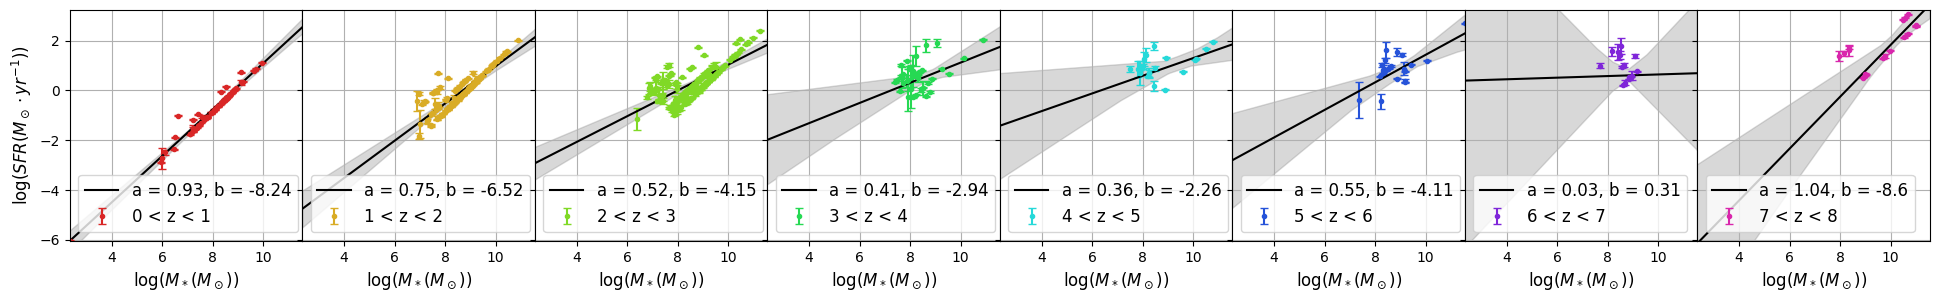
\includegraphics[width=1\textwidth]{assets/main_sequence_redshift.png}
  \caption{Séquence principale galactique en fonction du redshift. En raison du manque de discrétisations de la grille de paramètres, la dispersion des points est biaisée par rapport à leur dispersion réelle.}
  \label{fig:main_sequence}
\end{figure}

\begin{figure}[!h]
  \centering
  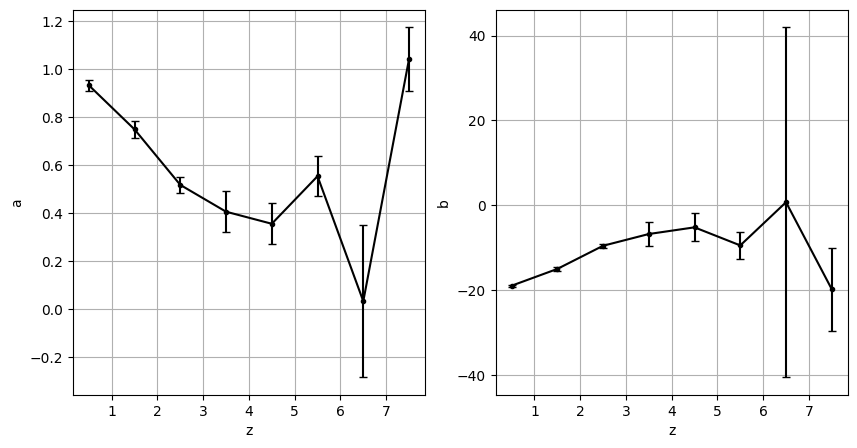
\includegraphics[width=0.8\textwidth]{assets/coeff_main_sequence.png}
  \caption{Evolution du coefficient directeur $a$ et de l'ordonnée à l'origine $b$ de la droite de meilleur ajustement (la puissance de la loi de puissance et un facteur multiplicatif) en fonction du redshift $z$. On remarque, outre les redshifts les plus élevés, que la tendance est que la droite tende vers l'horizontal et que l'ordonnée à l'origine augmente avec le \textit{redshift}. Cela signifie qu'à mesure que l'on remonte dans le temps, le taux de formation stellaire dépend de moins en moins de la masse stellaire.}
  \label{fig:coeff_main_sequence}
\end{figure}

En ignorant les \textit{redshift} supérieurs à 5, pour lesquels les comportements des droites changent radicalement en raison du nombre plus réduit de points, on peut alors tracer l'allure de chacune de ces droites et les comparer (\figref{fig:main_sequence_fit}) à des travaux antérieurs \parencite{10.1093_mnras_stac3214}.

En comparant nos modèles à la littérature, on observe que le comportement est similaire : à mesure que l'âge de l'univers augmente, la séquence principale est décalée vers le bas. Cela signifie donc que la formation stellaire était bien plus importante jadis qu'elle ne l'est maintenant.\\

\begin{figure}[!h]
  \centering
     \begin{subfigure}[t]{0.5\textwidth}
         \centering
         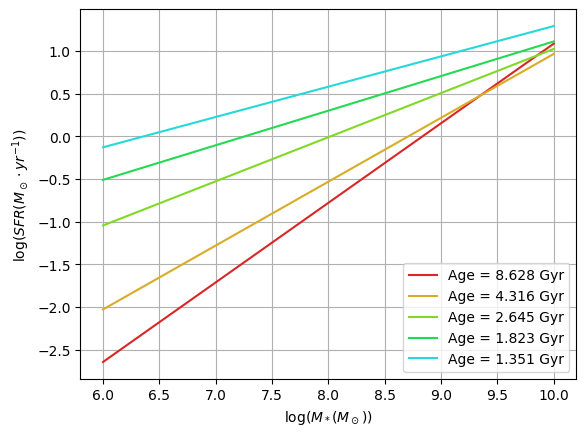
\includegraphics[width=\textwidth]{assets/main_sequence_fit.png}
         \caption{Droites modélisant la séquence principale à différents âges de l'univers. On a ici exclu les $z > 5$ en raison du manque de points.}
     \end{subfigure}
     \hfill
     \begin{subfigure}[t]{0.4\textwidth}
         \centering
         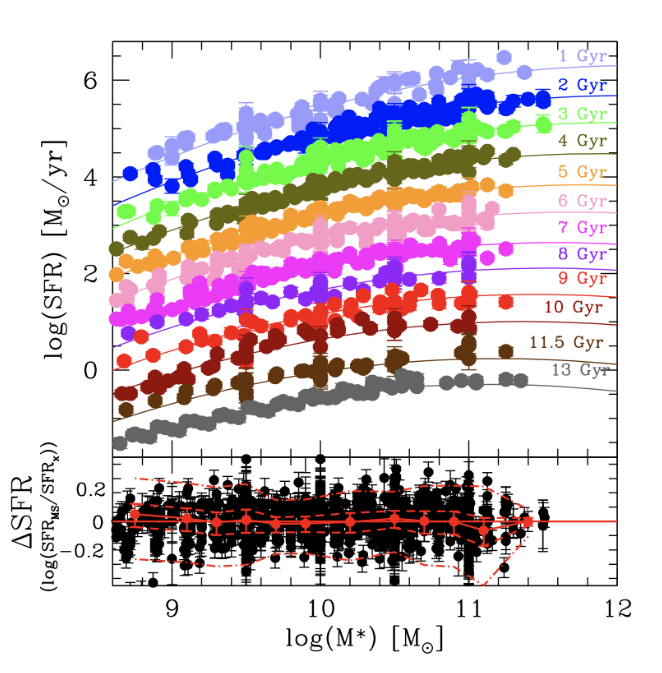
\includegraphics[width=\textwidth]{assets/main_sequence_theory.PNG}
         \caption{Modèles de la séquence principale tels que défini dans \cite{10.1093_mnras_stac3214}}
     \end{subfigure}
     \caption{}
     \label{fig:main_sequence_fit}
\end{figure}

On peut également tracer les différents indicateurs de métallicité en fonction du \textit{lookback time}, le temps de regard vers le passé, que l'on déduit avec le redshift et un modèle cosmologique. On affiche alors $Z_{gas}$ la métallicité du gaz et $Z_*$ la métallicité stellaire \figref{fig:metallicite_age}.

\begin{figure}[!h]
  \centering
  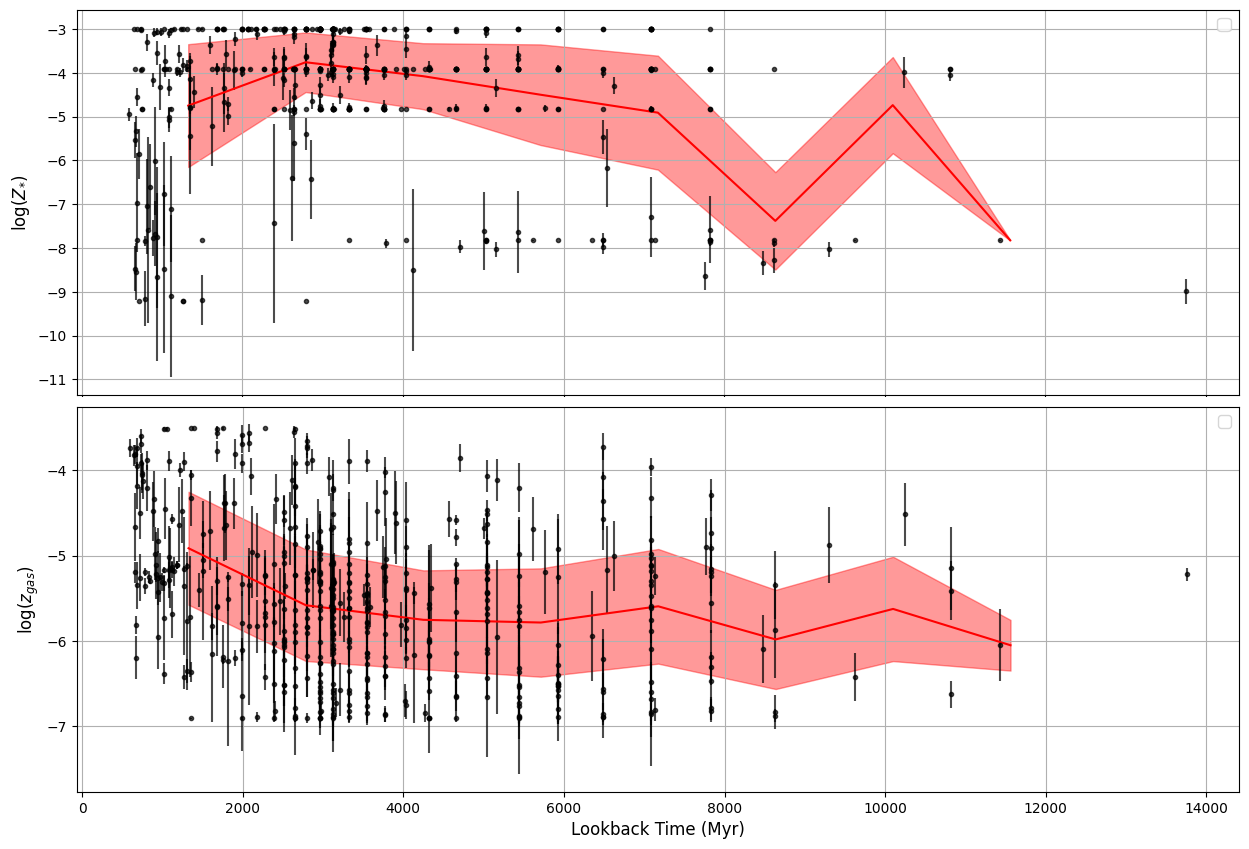
\includegraphics[width=1\textwidth]{assets/metallicite_w_age.png}
  \caption{Variation des différents indicateurs de métallicité en fonction du \textit{lookback time}. On remarque que l'on a bien, à mesure que l'on revient vers les origines de l'univers, une diminution de la métallicité avec $Z_*$ (la métallicité stellaire) et $Z_{gas}$ (la métallicité du gaz).}
  \label{fig:metallicite_age}
\end{figure}

Les fortes incertitudes observées sont potentiellement dûes aux erreurs d'ajustements relevés plus tôt. Une manière de s'en persuader est de s'intéresser aux \textit{mock} générés par \gls{cigale}. En effet, une fois le meilleur modèle trouvé pour un spectre donné, \gls{cigale} peut, à partir de ce modèle, simuler des données en ajoutant un bruit, dans l'objectif de vérifier si un paramètre donné est mesurable depuis la plage de longueur d'onde de nos observations. On peut alors tracer un graphique par paramètre, dans lesquels on place les valeurs estimées et les valeurs théoriques correspondantes. On affiche ces graphiques pour les indicateurs de métallicité sur la \figref{fig:mock_metallicity}

\begin{figure}[H]
  \centering
  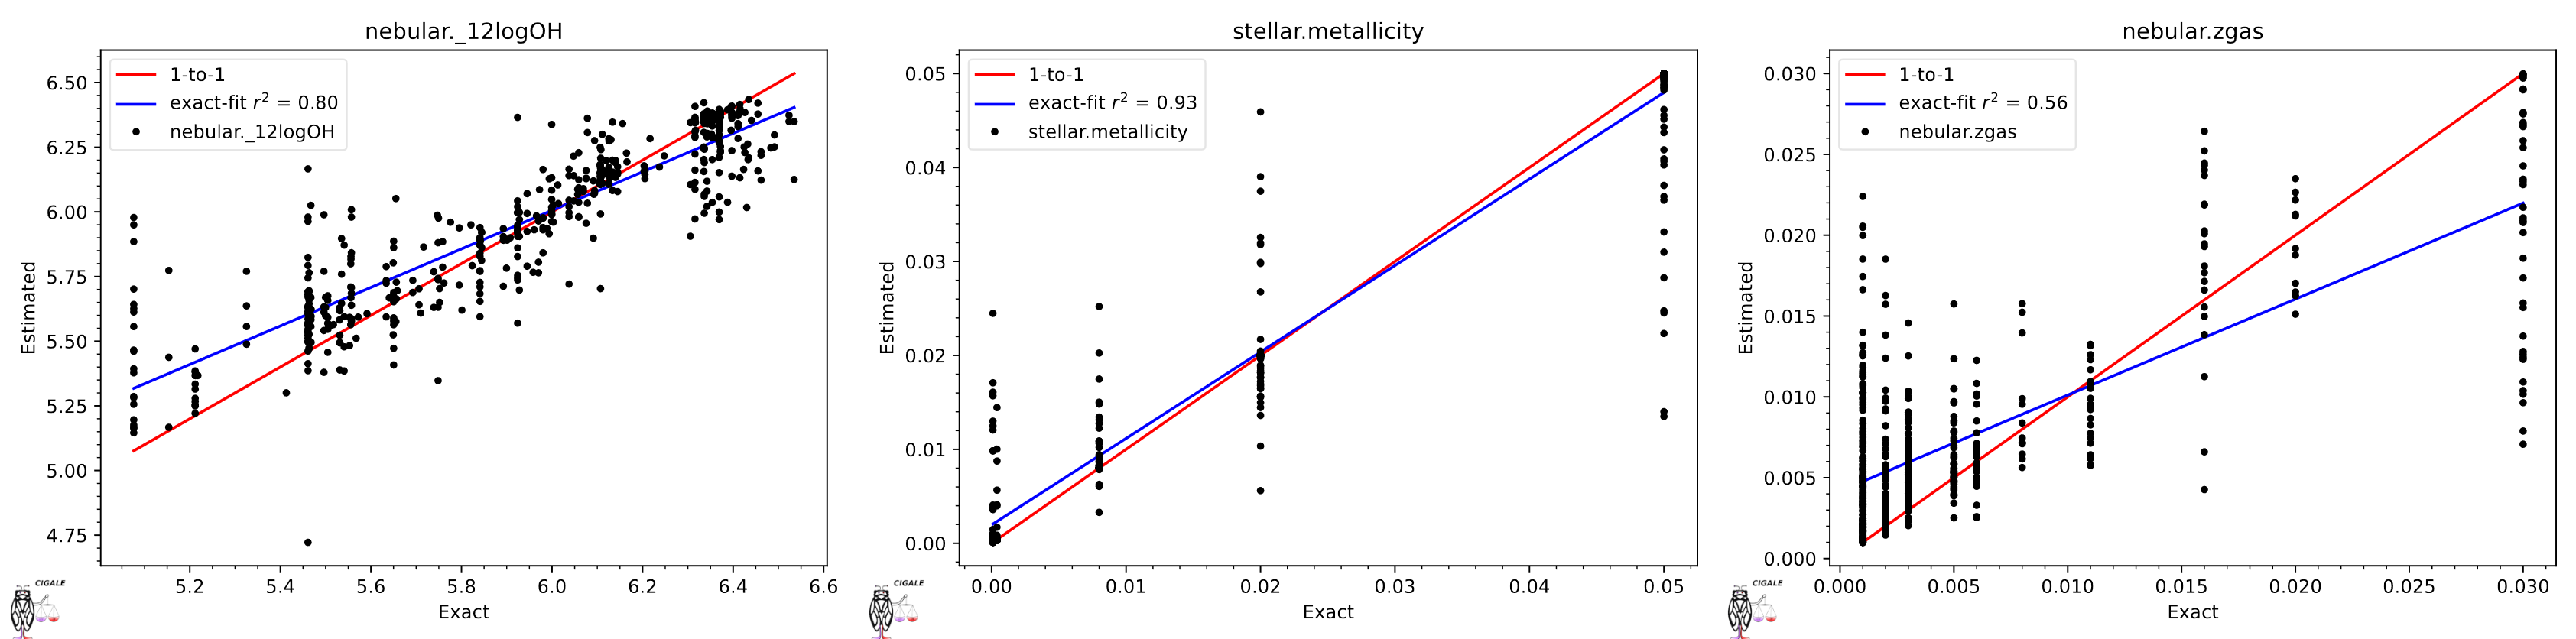
\includegraphics[width=1\textwidth]{assets/mock_metallicity.png}
  \caption{\textit{Mock} des 3 indicateurs de métallicité. Permet d'estimer la fiabilité de la détermination de chaque paramètre. On remarque que $z_{gas}$ n'est pas entièrement fiables (pente de $0.56$).}
  \label{fig:mock_metallicity}
\end{figure}


\section{Conclusion}

Ainsi nous avons pu établir une nouvelle méthode de soustraction du fond dans les observations spectroscopiques de \gls{nirspec}. Basée sur l'interpolation par une spline, celle-ci nous permet de récupérer des informations jusqu'alors dissimulées, à travers les sources secondaires se situant dans le champ de \gls{nirspec}.

Nous avons pu extraire ces sources primaires et secondaires et les étudier à l'aide de \gls{cigale}, qui nous permet de déterminer un modèle d'émission spectrale adapté pour chaque source.

Nous avons enfin pu extraire de ces modèles des paramètres physiques intéressants, tels que la métallicité, le taux de formation stellaire ou encore le redshift.\\

La principale contrainte durant ce travail fut la durée limitée de ce stage. En effet, nous n'avons pas pu autant entrer dans les détails de certains travaux initialement prévu. De façon non exhaustive, l'amélioration de l'ajustement du fond, la recherche de l'écart entre la qualité du signal sur bruit pour les données simulées par rapport aux données réelles, les ajustements avec \gls{cigale}, auraient pu bénéficier de temps supplémentaire. Ces différents points pourront néanmoins être revus durant ma thèse.

\newpage

\printnoidxglossaries

\newpage

\printbibliography %Prints bibliography

\newpage

\section{Annexe : pcigale.ini}
\label{pcigale.ini}

\verbatiminput{assets/pcigale.ini}

\end{document}
